\startchapter{Evaluation}
\label{chapter:evaluation}

\minitoc

% TODO Hausi: i) What is evaluated / what not / empirical? ii) Include eval and implementation details in every chapter — maybe in the summary box - or a paragraph/section? iii) Add an Appendix explaining the evaluation/implementation package (put everything on Github)

\glsreset{cmes}

This chapter presents the evaluation of our contributions. We conducted functional, experimental and qualitative validation of representative elements from each contribution. We do so based on the case studies introduced in  \cref{sect:overview--iac-case-study,sect:overview--suts-case-tudy}---\emph{Infrastructure Management Case Study} and \emph{Smart Urban Transit System Case study}. For the infrastructure management part, we present three application scenarios, namely: 1) assistance with acquisition of knowledge from deployed resources; 2) prevention of configuration drift for \gls{iac} templates; and 3) exploration of software architecture variants. Scenarios 1) and 2) (\cf{Section~\ref{subsect:evaluation--im-functional-validation}}) aim to validate the soundness and feasibility of our continuous software evolution pipeline. Scenario 3) aims to validate the capacity of our self-improvement feedback loop to contribute to the managed system's long-term evolution. For the smart transportation part, we present an application scenario focused on model identification and run-time adjustment (\cf{Section~\ref{subsect:evaluation--suts-functional-validation}}). Such a scenario aims to validate the soundness and feasibility of our run-time evolution reference architecture.

Our qualitative validation focuses on aspects not directly addressed by our infrastructure management case study. In Section~\ref{subsect:evaluation--im-qualitative-validation}, we address the following concerns: the holistic and continuous nature of our software evolution process; and our contribution to reduce remaining discontinuities in the \gls{sdlc}.

Since we introduced the case studies from the problem point of view, we state two concrete cases of application to conduct the evaluation. In the first case, we describe a \gls{cmes} based on the problem definition from Section~\ref{subsect:overview--iac-case-study-problem}. Similarly, in the second case, we follow the problem definition from Section~\ref{subsect:overview--suts-case-study-problem} to describe a transportation system. We model this system and conduct related experiments based on operation data from a Colombian \gls{brt} system.

%%%%%%%%%%%%%%%%%%%%
%
% IM Case Study
%
%%%%%%%%%%%%%%%%%%%%

\section{Infrastructure Management Case Study}
\label{sect:evaluation--infrastructure-management}

This section contains the validation of our contributions based on the infrastructure management case study. It is organized as follows. Section~\ref{subsect:evaluation--im-concrete-application} introduces our concrete case of application. Section~\ref{subsect:evaluation--im-functional-validation} presents the application scenarios concerning functional validation. Section~\ref{subsect:evaluation--im-experimental-validation} presents the application scenarios concerning experimental validation. Finally, Section~\ref{subsect:evaluation--im-qualitative-validation} addresses the qualitative validation of various aspects of our contributions.

\subsection{Concrete Case of Application: A Cloud Media Encoding Service}
\label{subsect:evaluation--im-concrete-application}

The \gls{cmes} features a \gls{rest} \gls{api} to convert digital media files from one standard format to another. Given an address of a website and a desired format, the \gls{cmes} will download any audio or video files present in the website and will convert them, if necessary. The catalog of supported websites contains more than a thousand news and media-sharing sites, including BBC, CBS, YouTube, Vimeo and SoundCloud. In case the site contains a playlist, the \gls{cmes} will collect the items and merge them into a single file. Requests to this service tend to be time consuming because they include establishing the connection, downloading the files, and compiling and encoding them if necessary. Users worldwide use similar services to download media files from social networks and websites, therefore, keeping the latency as low as possible is a priority, as well as maximizing the request-handling capacity.

The \gls{cmes} comprises two services: a \acrshort{grpc}-based\footnote{High-performance \gls{rpc} framework, available at \url{https://grpc.io}} worker component that downloads and converts the media files; and an \acrshort{http} front-end service (\ie{an \gls{api}}). We decided to deploy the \gls{cmes} using Kubernetes\footnote{Open-source system for automating deployment, scaling, and management of containerized applications, available at \url{https://kubernetes.io}} because it greatly facilitates realizing and enforcing deployment specifications. Moreover, it enables integrating third party components that are commonly required in a cloud environment, such as load balancing, caching, routing, rate limiting, and job handling.

\begin{figure}[h]
	\centering
	\includegraphics[width=0.4\columnwidth]{fig/evaluation/CMES-deployment.pdf}
	\caption{Deployment diagram for the bare minimum configuration of the \gls{cmes}}
	\label{fig:evaluation--im-CMES-deployment}
\end{figure}

We decided to start from a very simple architecture, suppressing any assumption regarding potential user traffic. The overall goal of our second contribution is that the software architecture and the computing infrastructure change along with the service demand. Figure~\ref{fig:evaluation--im-CMES-deployment} depicts the bare minimum configuration for the concrete application. \texttt{API} and \texttt{Worker} are Linux \emph{containers} assembled into one \emph{pod}---a group of one or more containers with shared storage and network. Service \texttt{media-encoding-svc} routes user requests from \texttt{http://domain.tld} to API through port 8080, and in turn to Worker through port 50051.

Resources of the computing infrastructure have been manually managed through the cloud provider's web dashboard. Nevertheless, it would be highly beneficial to manage them through \gls{iac} templates, using Terraform's \gls{hcl} notation. As expected, the \gls{cmes} is prone to the issues we discussed in Section~\ref{subsect:overview--iac-case-study-problem}, namely: migration from ad-hoc management to \gls{iac}, configuration drift (\ie{technical debt}), and the need for continuous improvement. The initial cluster configuration of the \gls{cmes} features a Kubernetes cluster with one control plane (\ie{a Kubernetes master node}) and three computing nodes. Each of them has been allocated 8 GB of \gls{ram} and 4 \glspl{vcpu}.

\subsection{Functional Validation}
\label{subsect:evaluation--im-functional-validation}

This section presents two application scenarios addressing the functional validation of our evolution pipeline. Section~\ref{subsubsect:evaluation--im-application-scenario-1} focuses on creating an \gls{iac} template and its corresponding instance from resources deployed to a target cloud environment. This scenario validates the feasibility of our model transformation chain, our \textsc{Fork and Collect} algorithm, and the integration of multiple software tools from the \gls{iac} life cycle. Section~\ref{subsubsect:evaluation--im-application-scenario-2} focuses on demonstrating how the pipeline handles changes on either side of the integration loop. This scenario validates the effectiveness of the direct and \gls{ci}-aware evolution workflows.

\subsubsection{Implementation Details}
\label{subsubsect:evaluation--im-implementation-details}

Our implementation of the continuous evolution pipeline is driven by run-time manipulation of models. We developed Historian's monitoring metamodel and Terraform's \gls{hcl} metamodel using Xcore\footnote{\url{https://wiki.eclipse.org/Xcore}}---a metamodeling \gls{dsl} based on Eclipse EMF.\footnote{\url{https://www.eclipse.org/modeling/emf}} On top of the \gls{hcl} metamodel, we developed an interpreter based on Eclipse Xtext.\footnote{\url{http://www.eclipse.org/Xtext}} The interpreter allows loading \gls{iac} templates and transforming them into \gls{hcl} model instances. Moreover, our interpreter's public \gls{api} allows comparing and merging \gls{hcl} models, as well as transforming them back to their textual representation. We implemented diff and merge functionalities based on EMF Compare.\footnote{\url{https://www.eclipse.org/emf/compare}}

We also developed a graph metamodel based on Java's \acrshort{xml} \gls{api}. We use this metamodel to configure Historian's endpoint dependencies. Listing~\ref{lst:evaluation--im-vmware-graph-configuration} depicts VMware's \gls{api} configuration tailored to our case of application. Each monitor declaration represents an \gls{http} GET endpoint. Their name references a unique identifier taken from VMware's OpenAPI model. To help developers specify the dependency graph, we developed a \gls{cli} tool for generating a base monitoring project, including authentication, logging and dependency configuration. This project is setup to use Historian's run-time library, thus requiring minimal effort from developers.

\begin{lstlisting}[style=xml,caption={Historian's configuration file for monitoring VMware resources},label=lst:evaluation--im-vmware-graph-configuration]
<?xml version="1.0" encoding="UTF-8" standalone="yes"?>
<monitors xmlns="http://www.rigiresearch.com/middleware/graph/1.0.0">
	<!-- VM details -->
	<monitor name="getVcenterVm">
		<input name="vm" source="listVcenterVm">vm</input>
		<mappings>
			<transformation selector="value"/>
			<augmentation inputs="vm"/>
		</mappings>
	</monitor>
	<!-- Datacenters details -->
	<monitor name="getVcenterDatacenter">
		<input name="datacenter" source="listVcenterDatacenter">datacenter</input>
		<mappings>
			<transformation selector="value"/>
			<augmentation inputs="datacenter"/>
		</mappings>
	</monitor>
	<!-- Inventory of datacenters -->
	<monitor name="listVcenterDatacenter">
		<output name="datacenter" selector="//datacenter" multivalued="true"/>
		<mappings>
			<transformation selector="//datacenter" multivalued="true"/>
		</mappings>
	</monitor>
	<!-- Inventory of VMs -->
	<monitor name="listVcenterVm">
		<input name="filter.vms">vm-22922</input>
		<output name="vm" selector="//vm" multivalued="true"/>
		<mappings>
			<transformation selector="//vm" multivalued="true"/>
		</mappings>
	</monitor>
	...
	<!-- Inventory of VMs per datacenter -->
	<monitor name="listVcenterVmFilteredByDatacenter" template="listVcenterVm">
		<input name="filter.datacenters" source="listVcenterDatacenter">datacenter</input>
		<mappings>
			<transformation selector="//vm" multivalued="true" groupByInput="filter.datacenters"/>
		</mappings>
	</monitor>
</monitors>
\end{lstlisting}

We managed the \gls{iac} template instances of our case of application through IBM~\gls{cam}. The communication between the evolution coordinator component from our pipeline and \gls{cam} was implemented by consuming \gls{cam}'s public \gls{rest} \gls{api}. This includes functionality to initialize, plan, refresh and update Terraform template instances. Similarly, the evolution coordinator consumed Github's Git \gls{api} for creating a local copy of the target repository (\ie{a clone}), and publishing new code branches.

We implemented the evolution coordinator and the run-time agent as independent executable components. The former publishes a POST endpoint to receive specification updates from the latter.

% C1
\subsubsection{Application Scenario 1: Assistance With Knowledge Acquisition}
\label{subsubsect:evaluation--im-application-scenario-1}

Since the infrastructure resources are already running on VMware, we focus on the generation of the corresponding \gls{iac} template files, as well as the creation of the instance on IBM~\gls{cam}. The first step consists of executing the evolution coordinator. As shown in the logs below, the coordinator clones the existing---but so far empty---repository where the template files will be stored (\cf{Line~2}). Then, the coordinator collects an authentication token from \gls{cam} for executing future requests. Finally, it starts an evolution service on port 5050 to receive specification updates from the run-time agent.

\begin{mdframed}[style=consolestyle]
	\vspace{0.3em}
	\begin{lstlisting}[style=console]
	(*@\bfseries\textcolor{white}{\$ ./coordinator-0.1.0/bin/coordinator}@*)
	TerraformRepository - Cloned repository https://github.com/company/cmes
	CamClient - Collected authentication token (CAM)
	Server - Started the evolution service (port 5050)
	\end{lstlisting}
	\vspace{-0.3em}
\end{mdframed}

The second step consists of executing the run-time agent. In this case, we have implemented a VMware agent that knows how to map changes from the cloud resources to the current \gls{hcl} model instance---so far non-existent. As shown in the listing below, once executed, the agent instantiates a Historian monitor, thus scheduling a task for running the \textsc{Fork and Collect} algorithm periodically.

\begin{mdframed}[style=consolestyle]
	\vspace{0.3em}
	\begin{lstlisting}[style=console]
	(*@\bfseries\textcolor{white}{\$ ./vmware.hcl.agent-0.1.0/bin/vmware.hcl.agent}@*)
	RuntimeAgent - Started the Historian Monitor
	\end{lstlisting}
	\vspace{-0.3em}
\end{mdframed}

The third step is automated and consists of running \textsc{Fork and Collect} to create a snapshot of the resources running on VMWare. The algorithm starts exploring the \gls{api} endpoints based on the dependency graph (\cf{Listing~\ref{lst:evaluation--im-vmware-graph-configuration}}). As shown in Line~1 of the listing below, the first endpoints inventory the running system. That is, they list existing cloud resources. Subsequent endpoints collect details for each listed entity (\ie{Lines~4,~8 and~9}).

\begin{mdframed}[style=consolestyle]
	\vspace{0.3em}
	\begin{lstlisting}[style=console]
	ForkAndCollectAlgorithm - Branches: 5 Endpoints: listVcenterHost, listVcenterDatacenter, listVcenterFolder, listVcenterResourcePool, listVcenterVm, listVcenterCluster
	ForkAndCollectAlgorithm - Branches: 1 Endpoints: listVcenterVmFilteredByHost
	ForkAndCollectAlgorithm - Branches: 3 Endpoints: listVcenterVmFilteredByDatacenter
	ForkAndCollectAlgorithm - Branches: 3 Endpoints: getVcenterDatacenter
	ForkAndCollectAlgorithm - Branches: 1 Endpoints: listVcenterVmFilteredByFolder
	ForkAndCollectAlgorithm - Branches: 5 Endpoints: listVcenterVmFilteredByResourcePool
	ForkAndCollectAlgorithm - Branches: 5 Endpoints: getVcenterResourcePool
	ForkAndCollectAlgorithm - Branches: 1 Endpoints: getVcenterVm
	ForkAndCollectAlgorithm - Branches: 3 Endpoints: getVcenterCluster
	\end{lstlisting}
	\vspace{-0.3em}
\end{mdframed}

The listing below depicts the \acrshort{json} document created by \textsc{Fork and Collect}. It contains the minimum amount of information necessary to instantiate or update the \gls{iac} model. The property names match those from the dependency graph, and in turn, the endpoint identifiers from VMware's OpenAPI specification.

\begin{lstlisting}[style=json]
{
	"listVcenterHost":[
		"host-112"
	],
	"listVmFilteredByHost":{
		"host-112":[
			"vm-22922"
		]
	},
	...
	"listVcenterDatacenter":[
		"CAMDC1",
		"CAMDC2"
	],
	"listVcenterVmFilteredByDatacenter":{
		"CAMDC1":[
			"vm-22922"
		],
		"CAMDC2":[]
	},
	"listVcenterVm":[
		"vm-22922"
	],
	"getVcenterVm":[
		{
			"vm":"vm-22922",
			...
			"cpu":{ ... },
			"disks":[ ... ],
			"memory":{ ... },
			"name":"camc-vis232c-vm-121"
		}
	],
	...
	"listVcenterResourcePool":{
		"value":[
			{
				"name":"CAM02/Resources",
				"resource_pool":"resgroup-1"
			}
		]
	}
}
\end{lstlisting}

Right after exploring VMware's \gls{api}, the agent maps the \acrshort{json} document to \gls{hcl} resources, thus instantiating a model that represents the current deployment. It also extracts parameter information from the document, including their name and current value on VMware. The agent finishes the scheduled task by sending both elements, the specification and the parameters, to the evolution coordinator. The parameters are created to match those present in the Terraform template, as well as those included in \gls{cam}'s instance.

\begin{mdframed}[style=consolestyle]
	\vspace{0.3em}
	\begin{lstlisting}[style=console]
	RuntimeAgent - Sent the current specification to the evolution coordinator
	RuntimeAgent - The specification values are as follows
	RuntimeAgent - (*@\textcolor{consolegreen}{resource\_pool\_1\_name}@*) = (*@\textcolor{consolegreen}{CAM02/Resources}@*)
	RuntimeAgent - (*@\textcolor{consolegreen}{vm\_1\_num\_cores\_per\_socket}@*) = (*@\textcolor{consolegreen}{1}@*)
	RuntimeAgent - (*@\textcolor{consolegreen}{vm\_1\_disk\_1\_unit\_number}@*) = (*@\textcolor{consolegreen}{0}@*)
	RuntimeAgent - (*@\textcolor{consolegreen}{vm\_1\_name}@*) = (*@\textcolor{consolegreen}{camc-vis232c-vm-121}@*)
	RuntimeAgent - (*@\textcolor{consolegreen}{vm\_1\_number\_of\_cpus}@*) = (*@\textcolor{consolegreen}{2}@*)
	RuntimeAgent - (*@\textcolor{consolegreen}{vm\_1\_adapter\_1\_type}@*) = (*@\textcolor{consolegreen}{VMXNET3}@*)
	RuntimeAgent - (*@\textcolor{consolegreen}{vm\_1\_scsi\_type}@*) = (*@\textcolor{consolegreen}{lsilogic}@*)
	RuntimeAgent - (*@\textcolor{consolegreen}{vm\_1\_guest\_os\_id}@*) = (*@\textcolor{consolegreen}{ubuntu64Guest}@*)
	RuntimeAgent - (*@\textcolor{consolegreen}{network\_1\_interface\_1\_label}@*) = (*@\textcolor{consolegreen}{VIS232}@*)
	RuntimeAgent - (*@\textcolor{consolegreen}{vm\_1\_disk\_1\_label}@*) = (*@\textcolor{consolegreen}{camc-vis232c-vm-121/camc-vis232c-vm-121.vdmk}@*)
	RuntimeAgent - (*@\textcolor{consolegreen}{datastore\_1\_name}@*) = (*@\textcolor{consolegreen}{CAM02-RSX6-002}@*)
	RuntimeAgent - (*@\textcolor{consolegreen}{vm\_1\_memory}@*) = (*@\textcolor{consolegreen}{2048}@*)
	RuntimeAgent - (*@\textcolor{consolegreen}{datacenter\_1\_name}@*) = (*@\textcolor{consolegreen}{CAMDC2}@*)
	RuntimeAgent - (*@\textcolor{consolegreen}{vm\_1\_disk\_1\_size}@*) = (*@\textcolor{consolegreen}{85}@*)
	RuntimeAgent - (*@\textcolor{consolegreen}{vm\_1\_folder}@*) = (*@\textcolor{consolegreen}{ContentRunTimes}@*)
	...
	\end{lstlisting}
	\vspace{-0.3em}
\end{mdframed}

The evolution coordinator uses the \gls{hcl} interpreter for merging the current model with the new one. In this case, since there is no current model, it just stores it. Next, it transforms the model into its textual representation and updates the local repository. In addition to the Terraform files, the coordinator also generates \texttt{camtemplate.json} and \texttt{camvariables.json}, two \acrshort{json} templates required to import the repository into \gls{cam}. These files contain information about the Terraform template, the repository, and declared parameters. Changes to the remote repository are included in a new branch by default.

\begin{mdframed}[style=consolestyle]
	\vspace{0.3em}
	\begin{lstlisting}[style=console]
	TerraformRepository - Pushed changes to the remote repository
	\end{lstlisting}
	\vspace{-0.3em}
\end{mdframed}

Having published the new template, the coordinator proceeds to import the template if it does not exist, specifying the repository and the new branch. Next, it creates an instance and performs various Terraform actions, as shown in the listing below. First, it performs a Terraform plan (\cf{Line~1}), which uses the VMware provider to analyze the deployed resources with respect to the template and the parameter values. As the status indicates, Terraform determines that some changes are necessary (\cf{Line~2}). This is because Terraform's current state is unaware that the specified resources are the same ones running on VMware. The coordinator then imports the resource identifiers into Terraform's state (\cf{Line~3}), and then confirms that the changes are no longer necessary (\cf{Line~6}). At the time our prototype was implemented, \gls{cam} did not support the import action. Therefore, we performed this action manually.

\begin{mdframed}[style=consolestyle]
	\vspace{0.3em}
	\begin{lstlisting}[style=console]
	CamClient - Started a Terraform plan
	CamClient - PLAN action ended with status SUCCESS_WITH_CHANGES
	CamClient - Started a Terraform import
	CamClient - IMPORT action ended with status SUCCESS
	CamClient - Started a Terraform plan
	CamClient - PLAN action ended with status SUCCESS
	\end{lstlisting}
	\vspace{-0.3em}
\end{mdframed}

Listing~\ref{lst:evaluation--im-vm-declaration} shows the contents of the Terraform template. It contains i) a list of variables declared from the collected resource attributes (\cf{Lines~1-4}); ii) provider and data declarations necessary to link the new Terraform resources with those outside the \gls{iac} life cycle (\cf{Lines~5-12}), such as data centers and hosts;\footnote{These resources are configured by the cloud provider, therefore they are not managed along with the \gls{cmes}'s resources.} and iii) the imported resources (\cf{Lines~13-49}).

\begin{lstlisting}[style=iac,caption={Declaration of VMware resources in the Terraform template},label=lst:evaluation--im-vm-declaration]
variable "datacenter_1_name" {
	type = "string"
}
...
provider "camc" {
	version = "~> 0.2"
}
...
data "vsphere_datacenter" "datacenter_1" {
	name = "${var.datacenter_1_name}"
}
...
resource "vsphere_virtual_machine" "vm_1" {
	datastore_id         = "${data.vsphere_datastore.datastore_1.id}"
	folder               = "${var.vm_1_folder}"
	guest_id             = "${var.vm_1_guest_os_id}"
	memory               = "${var.vm_1_memory}"
	name                 = "${var.vm_1_name}"
	num_cores_per_socket = "${var.vm_1_num_cores_per_socket}"
	num_cpus             = "${var.vm_1_number_of_cpus}"
	resource_pool_id     = "${data.vsphere_resource_pool.resource_pool_1.id}"
	scsi_type            = "${var.vm_1_scsi_type}"
	clone {
		template_uuid = "${data.vsphere_virtual_machine.vm_1_template.id}"
		customize {
			dns_server_list = "${var.vm_1_dns_servers}"
			dns_suffix_list = "${var.vm_1_dns_suffixes}"
			ipv4_gateway    = "${var.vm_1_ipv4_gateway}"
			linux_options {
				domain    = "${var.vm_1_domain}"
				host_name = "${var.vm_1_name}"
			}
			network_interface {
				ipv4_address = "${var.vm_1_ipv4_address}"
				ipv4_netmask = "${var.vm_1_ipv4_prefix_length}"
			}
		}
	}
	disk {
		label       = "${var.vm_1_disk_1_label}"
		size        = "${var.vm_1_disk_1_size}"
		unit_number = "${var.vm_1_disk_1_unit_number}"
	}
	network_interface {
		adapter_type = "${var.vm_1_adapter_1_type}"
		network_id   = "${data.vsphere_network.network_1.id}"
	}
}
...
\end{lstlisting}

In this section, we did a walkthrough of the first application scenario step by step. We showed how our prototype collects information from the target cloud and successfully creates the corresponding Terraform and \gls{cam} templates. Moreover, we describe additional interactions with \gls{cam} to instantiate the new template, thus closing the integration loop. Therefore, our prototype was able to acquire the necessary knowledge to migrate the \gls{cmes} from ad-hoc infrastructure management to \gls{iac}.

% C1
\subsubsection{Application Scenario 2: Prevention of Configuration Drift}
\label{subsubsect:evaluation--im-application-scenario-2}

This application scenario focuses on demonstrating that our integration loop prevents configuration drift. That is, we show that our loop keeps the artifacts from both sides (\ie{Dev and Ops}) synchronized. This includes the Terraform template, the \gls{cam} instance, and the deployed resources. In Section~\ref{subsubsect:evaluation--im-application-scenario-1}, we already showed the mapping process from Ops to Dev (\ie{from VMware to Terraform and \gls{cam}}). Therefore, in this section we focus on the updates stemming from changes on either side.

From left to right, changes can be either structural or parametric. In the first case, changes would occur in the Terraform specification. Nevertheless, for this change to be eventually deployed, the template instance needs to be updated first on \gls{cam}. Changing the template is a conscious and intentional effort. This means that changing the corresponding instance is expected to follow. In any case, modifying the template without reflecting the changes on \gls{cam} would have no effect on the instance or the deployed resources. Therefore, we do not consider this case as a potential drift in the configuration. In the second case, changes would occur on the template instance. Once the parameter values are updated, \gls{cam} performs a Terraform plan action followed up by an apply action. As a result, the cloud resources are synchronized with the template instance. Eventually, the Historian monitor will notify the run-time agent about the changes, and in turn, the agent will notify the evolution coordinator. However, since the template did not change, it only updates the values, as shown in the logs below.

\begin{mdframed}[style=consolestyle]
	\vspace{0.3em}
	\begin{lstlisting}[style=console]
	RuntimeAgent - The specification did not change
	RuntimeAgent - The specification values are as follows
	RuntimeAgent - resource_pool_1_name = CAM02/Resources
	RuntimeAgent - vm_1_num_cores_per_socket = 1
	RuntimeAgent - vm_1_disk_1_unit_number = 0
	RuntimeAgent - vm_1_name = camc-vis232c-vm-121
	RuntimeAgent - vm_1_number_of_cpus = 2
	RuntimeAgent - vm_1_adapter_1_type = VMXNET3
	RuntimeAgent - vm_1_scsi_type = lsilogic
	RuntimeAgent - vm_1_guest_os_id = ubuntu64Guest
	RuntimeAgent - network_1_interface_1_label = VIS232
	RuntimeAgent - vm_1_disk_1_label = camc-vis232c-vm-121/camc-vis232c-vm-121.vdmk
	RuntimeAgent - datastore_1_name = CAM02-RSX6-002
	RuntimeAgent - vm_1_memory = (*@\bfseries\textcolor{red}{2048}@*) -> (*@\bfseries\textcolor{consolegreen}{4096}@*)
	RuntimeAgent - datacenter_1_name = CAMDC2
	RuntimeAgent - vm_1_disk_1_size = (*@\bfseries\textcolor{red}{85}@*) -> (*@\bfseries\textcolor{consolegreen}{120}@*)
	RuntimeAgent - vm_1_folder = ContentRunTimes
	...
	\end{lstlisting}
	\vspace{-0.3em}
\end{mdframed}

The coordinator starts a new Terraform plan, which ends successfully without requiring further actions. At this point, both sides are effectively synchronized.

\begin{mdframed}[style=consolestyle]
	\vspace{0.3em}
	\begin{lstlisting}[style=console]
	CamClient - Started a Terraform plan
	CamClient - PLAN action ended with status SUCCESS
	\end{lstlisting}
	\vspace{-0.3em}
\end{mdframed}

From right to left, changes can originate from multiple sources, such as a web management dashboard, a \gls{cli} tool, a script, or the cloud infrastructure itself (\eg{an automated migration}). In any case, it is very likely that the change will be ultimately performed through the cloud's public \gls{api}. Therefore, for testing our prototype, it is enough with choosing only one source. We performed a storage migration using VMware's migration tool from the web dashboard. Consequently, the run-time agent identifies the migration and sends the new data store to the evolution coordinator. The listing below shows the output logs from the run-time agent. As in the previous case, the evolution coordinator updates the parameter on \gls{cam}, and the transaction ends with a successful Terraform plan.

\begin{mdframed}[style=consolestyle]
	\vspace{0.3em}
	\begin{lstlisting}[style=console]
	RuntimeAgent - The specification did not change
	RuntimeAgent - The specification values are as follows
	RuntimeAgent - resource_pool_1_name = CAM02/Resources
	...
	RuntimeAgent - vm_1_guest_os_id = ubuntu64Guest
	RuntimeAgent - network_1_interface_1_label = VIS232
	RuntimeAgent - vm_1_disk_1_label = camc-vis232c-vm-121/camc-vis232c-vm-121.vdmk
	RuntimeAgent - datastore_1_name = (*@\bfseries\textcolor{red}{CAM02-RSX6-002}@*) -> (*@\bfseries\textcolor{consolegreen}{visidpxer18\_local}@*)
	RuntimeAgent - vm_1_memory = 4096
	...
	\end{lstlisting}
	\vspace{-0.3em}
\end{mdframed}

There is a last type of run-time change that may cause configuration drift. In the event that a cloud resource is deleted, or added to Historian's monitoring configuration,\footnote{This is possible by updating the VMware \acrshort{xml} configuration. More specifically, the endpoint filters need be updated, and the run-time agent must be re-executed.} both the template and its instances need be reassessed. As shown in Section~\ref{subsubsect:evaluation--im-application-scenario-2}, the evolution coordinator will add new resources to the Terraform template, as well as their corresponding variables, providers, and data declarations. Since this functionality is based on model-to-text transformations, deleting resources would work as well. The coordinator creates a new version for each instance pointing to the new repository branch. This means that a member of the team needs to approve the new versions manually.

In this section, we have covered various evolution scenarios. We discussed how our integration loop, through round-trip engineering, contributes to reduce configuration drift for deployments managed with Terraform and \gls{cam}. In the next section, we concentrate on the experimental validation of our contributions.

\subsection{Experimental Validation of Our Proof of Concept}
\label{subsect:evaluation--im-experimental-validation}

%Our experimental validation for the infrastructure management case study consists of two parts. First, Section~\ref{subsubsect:evaluation--im-application-scenario-3} reports on a semi-automated exploration of software architecture variants (\ie{Our implementation of the~\gls{cfl}}). We aim to show how architecture variants perform under distinct execution scenarios. Thereby, we demonstrate the feasibility of our experimentation feedback loop. Moreover, we show the relevance of recognizing what configurations perform best according to specific software qualities. In this case, we focus on service latency. Second, Section~\ref{subsubsect:evaluation--im-application-scenario-4} reports on a similar exploration, but this time focused on the computing cluster (\ie{Our implementation of the~\gls{pfl}}). We show how the \gls{pfl} can find a cost-effective cluster configuration that meets a required service latency. Our findings are consistent with our contribution's purpose: the computing infrastructure and the software architecture must co-evolve, continuously, to meet changing requirements. By performing these explorations during development, autonomic decisions at run-time are timely, but also cost-effective. Moreover, our implementations of the \gls{cfl} and \gls{pfl} found performant variants that meet the required service latency. Therefore, they are able to contribute long-lasting changes to the evolution of the managed system, in a continuous way.

%\subsection{Application Scenario 3: Exploration of Software Architecture Variants}
%\label{subsubsect:evaluation--im-application-scenario-3}

The experimental validation of our proof of concept, for the infrastructure management case study, consists of a semi-automated exploration of software architecture variants (\ie{Our implementation of the~\gls{cfl}}). We aim to show how architecture variants perform under distinct execution scenarios. Thereby, we demonstrate the feasibility of our experimentation feedback loop. Moreover, we show the relevance of recognizing what configurations perform best according to specific software qualities. In this case, we focus on service latency. By performing this exploration during development, autonomic decisions at run-time are timely, but also cost-effective. Moreover, our prototype implementation found performant variants that meet the required service latency. Therefore, they are able to contribute long-lasting changes to the evolution of the managed system, in a continuous way.

This section is structured as follows. We first detail some aspects of our implementation in Section~\ref{par:evaluation--im-architecture-experimental-implementation}. We then describe the experimentation setup in Section~\ref{par:evaluation--im-architecture-experimental-setup}. Finally, we present and analyze the results in Section~\ref{par:evaluation--im-architecture-experiment-results}. In this section, we omit some of the charts depicting the behavior of each architecture variant. These additional resources are included in Appendix~\ref{appendix:additional-charts}.

\subsubsection{Implementation Details}
\label{par:evaluation--im-architecture-experimental-implementation}

Our implementation of the \gls{cfl} takes advantage of Kubernetes's declarative configuration for devising architecture variants. We built a library of design patterns by manipulating manifest files---that is, Kubernetes's specifications. Figure~\ref{fig:evaluation--im-kubedsl-manifest} displays a simplified version of the Kubernetes manifest for the bare minimum configuration of the \gls{cmes}. The constituent elements of the manifest file match those present in Figure~\ref{fig:evaluation--im-kubedsl-axes}. Such a figure depicts the relationships between Kubernetes resources declared in the manifest. Each of these relationships represents an axis for navigating forward and backward from any given resource. For example, given any container, it is possible to navigate to its containing pod and, in turn, navigate to the associated service or deployment. We used these navigation axes to implement our pattern library. Figure~\ref{fig:evaluation--im-kubedsl-implementation} contains a sample implementation of the Load Balancer pattern. Lines~8 and~9 refer to parameters associated with the pattern, whereas Lines~8-18 implement the actual pattern application. In this case, the implementation takes advantage of Kubernetes's built in load balancer for deployments, thus, setting the number of pod instances suffices for applying the pattern. The \gls{cfl} uses our library for loading and transforming manifest files before deploying the experiment trials.

\begin{figure}[h]
	\centering
	\begin{subfigure}[b]{0.65\textwidth}
		\centering
		\includegraphics[width=1\linewidth]{fig/evaluation/evaluation--im-kubedsl-manifest.pdf}
		\caption{Resource definitions}
		\label{fig:evaluation--im-kubedsl-manifest}
	\end{subfigure}
	%
	\begin{subfigure}[b]{0.64\textwidth}
		\centering
		\includegraphics[width=1\linewidth]{fig/evaluation/evaluation--im-kubedsl-axes.pdf}
		\caption{Abstract navigation axes}
		\label{fig:evaluation--im-kubedsl-axes}
		Circles represent Kubernetes resources. Arcs are navigation links for traversing the specification.
	\end{subfigure}
	\caption{Fluent interface for navigating Kubernetes resources}
	\label{fig:evaluation--im-kubedsl}
\end{figure}

\begin{figure}[h]
	\centering
	\includegraphics[width=0.9\textwidth]{fig/evaluation/evaluation--im-kubedsl-implementation.pdf}
	\caption{Sample pattern definition using our fluent interface}
	\label{fig:evaluation--im-kubedsl-implementation}
\end{figure}

To simplify the implementation, and because some design patterns contain application-specific code (\ie{Master/Worker and Producer/Consumer}), we tested 6 of the generated configurations. Although a complete run of the experiment would provide more accurate results, we believe that comparing these trials is representative of the overall results. Furthermore, these design variants are commonly found in production-ready applications with moderate workload. The variants are as follows.

\begin{description}[noitemsep,font=\bfseries\normalsize]
	% Cache-2
	\item[V1] Client$\shortra$Proxy-Cache$\shortra$LB$\shortra$API$\shortra$LB$\shortra$Worker
	% Cache-3.2
	\item[V2] Client$\shortra$LB$\shortra$Proxy-Cache$\shortra$LB$\shortra$API$\shortra$LB$\shortra$Worker
	% Cache-3.1
	\item[V3] Client$\shortra$LB$\shortra$Proxy-Cache (sharded)$\shortra$LB$\shortra$API$\shortra$LB$\shortra$Worker
	\item[V4] Client$\shortra$Rate-Limiting-Proxy$\shortra$LB$\shortra$API$\shortra$LB$\shortra$Worker
	\item[V5] Client$\shortra$API$\shortra$Master/Worker$\shortra$Worker
	\item[V6] Client$\shortra$API$\shortra$Producer/Consumer$\shortra$Worker
\end{description}

All variants load-balance requests to API and Worker. Variants V5 and V6 do so with an implicit load balancer. Variant V1 has a single Proxy Cache instance. Variant V2 is similar but it contains a cache cluster. We duplicated this variant into V3 to measure the effect of sharding the cache. All Proxy Cache instances implemented the same caching policy: The request \acrshort{url} was used as the cache key; Revalidation was set to off, and a minimum use of 0 requests was required to store responses in the cache; And cache lock was enabled with an age of 30 seconds and timeout of 60 seconds. Similarly, all instances of Load Balancer used the same number of container instances: 10 for API, 15 for Worker, and 10 for Proxy Cache. In the case of Master/Worker there were 10 instances of the Master component. And for Producer/Consumer, there were 10 producer and consumer adapters.

\subsubsection{Experimentation Setup}
\label{par:evaluation--im-architecture-experimental-setup}

We used load testing to simulate predictable user traffic according to three execution scenarios, namely: Regular, Linear and Spike. The Regular scenario represents a stable user traffic with a target throughput of 450 requests distributed across 30 users (\ie{threads}). The Spike scenario was set up similarly targeting 150 requests with an additional spike of 90 requests. And the Linear scenario represents an increasing user traffic of 160 users with a ramp-up period of 1 second. Experiment results ended up containing fewer requests due to the hosting platform (\ie{YouTube}) restricting the number of consecutive requests. Nevertheless, sample sizes are large enough to guarantee sound analyses. Each scenario was modeled using jMeter,\footnote{\url{https://jmeter.apache.org}} which allowed us to have repeatable executions and measurements per request. The scenarios were executed on a single machine with 8 GB of \gls{ram} and a 1.6 GHz Dual-Core Intel i5 processor. The Kubernetes cluster was setup based on the \gls{cmes}'s initial configuration (\ie{3 computing nodes with 8 GB of \gls{ram} and 4 \glspl{vcpu}}). % The Kubernetes cluster contained three worker nodes, each with 8 GB of \gls{ram} and 4 \glspl{vcpu}.
Load balancing for \gls{http} was done with nginx,\footnote{\url{https://nginx.org}} and linkerd\footnote{\url{https://linkerd.io}} for \acrshort{grpc}. Each scenario ran for at least 5 minutes.

The test data was created based on a catalog of 80 videos and 80 playlists, which were uploaded to YouTube. The latter contains 10 videos each from the former. Although there were 80 different \acrshort{url}s, it is worth noting that all of them corresponded to the same 2 minute and 2.6 MB video. We made this decision aiming to reduce the variability in the results.

\subsubsection{Experimentation Results}
\label{par:evaluation--im-architecture-experiment-results}

The Shapiro-Wilk test confirmed that none of the variants' samples are normal. The Kruskal-Wallis test found a significant difference in the mean latencies for all scenarios. According to Dunn's test, variants V1, V2 and V3 are not significantly different for any of the scenarios, regardless of the request type. For the Regular scenario and video requests, Dunn's test found that V4 and V6 are different by chance. In the case of playlist requests, the test found that V4, V5 and V6 are not significantly different. Out of these variants, V3 was selected as the best one\footnote{We averaged video and playlist requests and chose the smallest out of the cluster containing V1, V2 and V3.} with a mean latency of 1.46 seconds for videos and 1.62 seconds for playlists. We present various descriptive statistics for video and playlist requests in Table~\ref{tab:evaluation--im-mean-latencies}. Table~\ref{tab:evaluation--im-dunn-test} displays pairwise comparisons from Dunn's test for video and playlist requests. The Z statistic represents how many standard deviations, above or below, is the z-test from the mean population from which the score derived. That is, it describes each latency value's relationship to the mean of the group. In a multiple comparison testing, the adjusted P value is the smallest (familywise) significance level at which a particular comparison will be declared statistically significant. Figure~\ref{fig:evaluation--im-architecture-regular-latency-by-request-type} shows the latency by request type for the Regular scenario.

\begin{table}[p]
	\centering
	\caption{Descriptive statistics for video and playlist requests}
	{\emph{n} represents the sample size, excluding erroneous requests, which appear in parenthesis; \emph{SD} and \emph{SE} stand for standard deviation and error; \emph{LCL} and \emph{UCL} stand for lower and upper control limits; \emph{Med} stands for median; \emph{Min} and \emph{Max} stand for minimum and maximum. Latency values are in seconds.\\ [0.3cm]}
	\label{tab:evaluation--im-mean-latencies}
	\begin{adjustbox}{center}
		\begin{tabular}{
				>{\scriptsize}r
				>{\scriptsize}r >{\scriptsize}r >{\scriptsize}r >{\scriptsize}r >{\scriptsize}r >{\scriptsize}r
				| >{\scriptsize}r >{\scriptsize}r >{\scriptsize}r >{\scriptsize}r >{\scriptsize}r >{\scriptsize}r
			}
			\toprule
			& \multicolumn{6}{c}{\normalsize\textbf{Video Requests}} &
			\multicolumn{6}{c}{\normalsize\textbf{Playlist Requests}} \\
			\midrule
			& V1 & V2 & V3 & V4 & V5 & V6 &
			V1 & V2 & V3 & V4 & V5 & V6 \\
			\hline
			\multicolumn{13}{c}{\scriptsize Regular} \\
			\hline
			
			n & 148 & 156 & 163 & 163 & 144 & 130 &
			160 & 152 & 145 & 132 (13) & 133 & 136 \\
			Mean & 1.65 & 1.61 & 1.46 & 4.03 & 13.5 & 12.2 &
			1.55 & 1.59 & 1.62 & 25.6 & 39.5 & 35.9 \\
			SD & 1.55 & 1.53 & 1.54 & 1.82 & 10.1 & 19.7 &
			1.52 & 1.54 & 1.56 & 11.5 & 23.2 & 23.7 \\
			SE & 0.127 & 0.123 & 0.121 & 0.143 & 0.842 & 1.73 &
			0.120 & 0.125 & 0.129 & 1.00 & 2.01 & 2.03 \\
			LCL & 1.40 & 1.37 & 1.22 & 3.75 & 11.8 & 8.79 &
			1.31 & 1.35 & 1.36 & 23.6 & 35.5 & 31.9 \\
			UCL & 1.91 & 1.85 & 1.70 & 4.31 & 15.1 & 15.6 &
			1.79 & 1.84 & 1.87 & 27.6 & 43.4 & 39.9 \\
			Med & 0.224 & 0.186 & 0.179 & 3.58 & 9.55 & 3.11 &
			0.182 & 0.181 & 0.199 & 24.6 & 32.9 & 28.4 \\
			Min & 0.153 & 0.152 & 0.158 & 1.46 & 4.78 & 2.05 &
			0.151 & 0.154 & 0.159 & 2.29 & 8.77 & 13.3 \\
			Max & 4.13 & 3.81 & 4.10 & 14.3 & 77.4 & 111 &
			3.82 & 3.97 & 3.97 & 60.8 & 108 & 127 \\
			
			\hline
			\multicolumn{13}{c}{\scriptsize Spike} \\
			\hline
			
			n & 101 & 84 & 93 & 72 (46) & 95 (4) & 84 &
			77 & 96 (4) & 85 (1) & 75 (44) & 59 (16) & 77 \\
			Mean & 9.86 & 6.95 & 9.87 & 4.45 & 98.2 & 63.8 &
			42.5 & 39.8 & 45.2 & 28.9 & 182 & 84.1 \\
			SD & 7.58 & 5.38 & 7.51 & 1.40 & 64.6 & 56.5 &
			25.1 & 29.5 & 34.2 & 11.9 & 80.7 & 50.8 \\
			SE & 0.754 & 0.587 & 0.779 & 0.165 & 6.62 & 6.16 &
			2.86 & 3.01 & 3.71 & 1.37 & 10.5 & 5.79 \\
			LCL & 8.36 & 5.78 & 8.32 & 4.12 & 85.0 & 51.6 &
			36.8 & 33.8 & 37.8 & 26.2 & 161 & 72.6 \\
			UCL & 11.4 & 8.11 & 11.4 & 4.78 & 111 & 76.1 &
			48.2 & 45.7 & 52.6 & 31.7 & 203 & 95.7 \\
			Med & 8.39 & 6.59 & 9.16 & 4.20 & 100 & 55.7 &
			46.1 & 38.9 & 40.6 & 27.5 & 200 & 80.4 \\
			Min & 0.241 & 0.238 & 0.241 & 2.19 & 4.11 & 2.58 &
			0.235 & 0.227 & 0.203 & 11.9 & 8.70 & 14.1 \\
			Max & 27.7 & 16.4 & 25.3 & 7.23 & 262 & 188 &
			90.5 & 121 & 121 & 59.8 & 293 & 196 \\
			
			\hline
			\multicolumn{13}{c}{\scriptsize Linear} \\
			\hline
			
			n & 84 (1) & 78 & 77 & 77 & 78 & 72 &
			72 (3) & 82 & 82 (1) & 79 (4) & 82 & 88 \\
			Mean & 2.77 & 2.64 & 2.80 & 4.61 & 47.8 & 50.5 &
			22.5 & 22.7 & 20.7 & 27.7 & 148 & 81.9 \\
			SD & 2.08 & 1.85 & 1.96 & 1.66 & 47.6 & 42.0 &
			17.2 & 18.2 & 16.4 & 10.9 & 55.8 & 43.6 \\
			SE & 0.227 & 0.210 & 0.223 & 0.190 & 5.39 & 4.95 &
			2.02 & 2.01 & 1.81 & 1.22 & 6.17 & 4.65 \\
			LCL & 2.32 & 2.22 & 2.36 & 4.23 & 37.1 & 40.6 &
			18.5 & 18.7 & 17.1 & 25.3 & 136 & 72.7 \\
			UCL & 3.22 & 3.06 & 3.24 & 4.99 & 58.5 & 60.4 &
			26.6 & 26.7 & 24.3 & 30.1 & 160 & 91.2 \\
			Med & 3.29 & 3.08 & 3.26 & 4.16 & 21.8 & 42.9 &
			24.8 & 23.6 & 20.0 & 24.6 & 156 & 71.9 \\
			Min & 0.228 & 0.237 & 0.246 & 2.15 & 4.18 & 2.86 &
			0.253 & 0.267 & 0.235 & 14.2 & 9.44 & 21.2 \\
			Max & 7.48 & 7.32 & 7.22 & 9.5 & 191 & 165 &
			89.9 & 59.6 & 60.4 & 59.1 & 271 & 176 \\
			
			\bottomrule
		\end{tabular}
	\end{adjustbox}
\end{table}

\begin{table}[p]
	\centering
	\caption{Pairwise comparisons from Dunn's test (Hochberg)}
	{Comparisons marked with a circle denote variants different by chance.\\ \vspace{0.3cm}}
	\label{tab:evaluation--im-dunn-test}
	\begin{tabular}{
			>{\scriptsize}r >{\scriptsize}r >{\scriptsize}l 
			| >{\scriptsize}r >{\scriptsize}r >{\scriptsize}l | 
			>{\scriptsize}r >{\scriptsize}r >{\scriptsize}l	
		}
		\toprule
		\multicolumn{3}{c}{\normalsize\textbf{Regular}} &
		\multicolumn{3}{c}{\normalsize\textbf{Spike}} &
		\multicolumn{3}{c}{\normalsize\textbf{Linear}} \\
		\midrule
		Variants & Z Statistic & Adj. P-value &
		Variants & Z Statistic & Adj. P-value &
		Variants & Z Statistic & Adj. P-value \\
		\hline
		\multicolumn{9}{c}{\scriptsize Video Requests} \\
		\hline
		$\bullet$ V1 - V3 & -0.137624 & 0.4453 &
		$\bullet$ V1 - V3 & -0.100347 & 0.4600 &
		$\bullet$ V1 - V3 & -0.191831 & 0.4239  \\
		$\bullet$ V1 - V2 & 0.809712 & 0.6272  &
		$\bullet$ V1 - V2 & 1.838233 & 0.0990 &
		$\bullet$ V1 - V2 & 0.588189 & 0.8346  \\
		$\bullet$ V3 - V2 & 0.969048 & 0.6650 &
		$\bullet$ V3 - V2 & 1.899160 & 0.1151 &
		$\bullet$ V3 - V2 & 0.764121 & 0.8896  \\
		V1 - V5 & -16.16428 & 0.0000* &
		V1 - V5 & -9.168365 & 0.0000* &
		V1 - V5 & -11.08871 & 0.0000* \\
		V3 - V5 & -16.40741 & 0.0000* &
		V3 - V5 & -8.884146 & 0.0000* &
		V3 - V5 & -10.66532 & 0.0000* \\
		V2 - V5 & -17.17664 & 0.0000* &
		V2 - V5 & -10.56171 & 0.0000* &
		V2 - V5 & -11.46649 & 0.0000* \\
		V1 - V6 & -7.520797 & 0.0000* &
		V1 - V6 & -5.815485 & 0.0000* &
		V1 - V6 & -11.19946 & 0.0000* \\
		V3 - V6 & -7.555149 & 0.0000* &
		V3 - V6 & -5.609327 & 0.0000* &
		V3 - V6 & -10.78703 & 0.0000* \\
		V2 - V6 & -8.395024 & 0.0000* &
		V2 - V6 & -7.324578 & 0.0000* &
		V2 - V6 & -11.57171 & 0.0000* \\
		V5 - V6 & 8.166741 & 0.0000* &
		V5 - V6 & 3.015430 & 0.0064* &
		$\bullet$ V5 - V6 & -0.336892 & 0.7362  \\
		V1 - V4 & -8.222174 & 0.0000* &
		V1 - V4 & 3.210086 & 0.0040* &
		V1 - V4 & -3.517963 & 0.0013* \\
		V3 - V4 & -8.286863 & 0.0000* &
		V3 - V4 & 3.245992 & 0.0041* &
		V3 - V4 & -3.256100 & 0.0028* \\
		V2 - V4 & -9.164485 & 0.0000* &
		$\bullet$ V2 - V4 & 1.392711 & 0.1637 &
		V2 - V4 & -4.030708 & 0.0002* \\
		V5 - V4 & 8.381079 & 0.0000* &
		V5 - V4 & 11.55495 & 0.0000* &
		V5 - V4 &  7.398736 & 0.0000* \\
		$\bullet$ V6 - V4 & -0.251111 & 0.8017 &
		V6 - V4 & 8.429938 & 0.0000* &
		V6 - V4 &  7.586034 & 0.0000* \\
		\hline
		\multicolumn{9}{c}{\scriptsize Playlist Requests} \\
		\hline
		$\bullet$ V1 - V3 & 0.465367 & 0.6417 &
		$\bullet$ V1 - V3 & 0.464571 & 0.3211 &
		$\bullet$ V1 - V3 & 0.465367 & 0.6417  \\
		$\bullet$ V1 - V2 & -0.076362 & 0.4696  &
		$\bullet$ V1 - V2 & 1.310816 & 0.2849 &
		$\bullet$ V1 - V2 & -0.076362 & 0.4696  \\
		$\bullet$ V3 - V2 & -0.560224 & 0.8630 &
		$\bullet$ V3 - V2 & 0.855698 & 0.3922 &
		$\bullet$ V3 - V2 & -0.560224 & 0.8630  \\
		V1 - V5 & -11.21401 & 0.0000* &
		V1 - V5 & -7.574920 & 0.0000* &
		V1 - V5 & -11.21401 & 0.0000* \\
		V3 - V5 & -12.07811 & 0.0000* &
		V3 - V5 & -8.165797 & 0.0000* &
		V3 - V5 & -12.07811 & 0.0000* \\
		V2 - V5 & -11.51788 & 0.0000* &
		V2 - V5 & -9.134892 & 0.0000* &
		V2 - V5 & -11.51788 & 0.0000* \\
		V1 - V6 & -8.186793 & 0.0000* &
		V1 - V6 & -3.867309 & 0.0004* &
		V1 - V6 & -8.186793 & 0.0000* \\
		V3 - V6 & -8.965656 & 0.0000* &
		V3 - V6 & -4.426219 & 0.0000* &
		V3 - V6 & -8.965656 & 0.0000* \\
		V2 - V6 & -8.395631 & 0.0000* &
		V2 - V6 & -5.384961 & 0.0000* &
		V2 - V6 & -8.395631 & 0.0000* \\
		V5 - V6 & 3.323748 & 0.0031* &
		V5 - V6 & 3.972616 & 0.0003* &
		V5 - V6 &  3.323748 & 0.0031* \\
		$\bullet$ V1 - V4 & -1.119305 & 0.6575 &
		V1 - V4 & 3.336781 & 0.0025* &
		$\bullet$ V1 - V4 & -1.119305 & 0.6575 \\
		$\bullet$ V3 - V4 & -1.633566 & 0.3070 &
		V3 - V4 & 2.955713 & 0.0078* &
		$\bullet$ V3 - V4 & -1.633566 & 0.3070 \\
		$\bullet$ V2 - V4 & -1.078586 & 0.5615 &
		$\bullet$ V2 - V4 & 2.211481 & 0.0540 &
		$\bullet$ V2 - V4 & -1.078586 & 0.5615 \\
		V5 - V4 & 10.33148 & 0.0000* &
		V5 - V4 & 10.64232 & 0.0000* &
		V5 - V4 & 10.33148 & 0.0000* \\
		V6 - V4 & 7.217215 & 0.0000* &
		V6 - V4 & 7.178564 & 0.0000* &
		V6 - V4 & 7.217215 & 0.0000* \\
		\bottomrule
	\end{tabular}
\end{table}

A similar analysis for the Spike scenario reveals that variants V2 and V4 are different by chance. Nevertheless, the number of erroneous requests for V4 clearly separates them. V4 rejected the requests causing the spike---a surge of at least 44 requests, which would be considered an abusive use of the \gls{cmes}. Consequently, V4 was selected as the best variant with a mean latency of 4.45 seconds for videos and 28.9 for playlists. Figure~\ref{fig:evaluation--im-architecture-spike-latency-by-request-type} shows the latency by request type for the Spike scenario. Figure~\ref{fig:evaluation--im-architecture-spike-latency-rate-limiting-proxy} shows that V4 completely mitigated the traffic spike, while the rest struggled to keep the latency low, even when caching the responses.

For the Linear scenario and video requests, variants V5 and V6 were found not significantly different. For playlist requests, variants V1, V2, V3 and V4 were found different by chance. These results are shown in Figure~\ref{fig:evaluation--im-architecture-linear-latency-by-request-type}. V3 was selected as the best variant with a mean latency of 2.80 seconds for videos and 20.7 for playlists.

\begin{figure}[p]
	\centering
	\begin{subfigure}[b]{0.48\textwidth}
		\includegraphics[width=1\linewidth]{fig/evaluation/architectural-framework/software-variants/regular/latency_type_Cache-2.pdf}
		\caption{V1}
		\label{fig:evaluation--im-architecture-regular-latency-cache-1}
	\end{subfigure}
	%
	\begin{subfigure}[b]{0.48\textwidth}
		\includegraphics[width=1\linewidth]{fig/evaluation/architectural-framework/software-variants/regular/latency_type_Cache-3_2.pdf}
		\caption{V2}
		\label{fig:evaluation--im-architecture-regular-latency-cache-2}
	\end{subfigure}
	%
	\begin{subfigure}[b]{0.48\textwidth}
		\includegraphics[width=1\linewidth]{fig/evaluation/architectural-framework/software-variants/regular/latency_type_Cache-3_1.pdf}
		\caption{V3}
		\label{fig:evaluation--im-architecture-regular-latency-cache}
	\end{subfigure}
	%
	\begin{subfigure}[b]{0.48\textwidth}
		\includegraphics[width=1\linewidth]{fig/evaluation/architectural-framework/software-variants/regular/latency_type_Rate-Limiting-Proxy.pdf}
		\caption{V4}
		\label{fig:evaluation--im-architecture-regular-latency-rate-limiting-proxy}
	\end{subfigure}
	%
	\begin{subfigure}[b]{0.48\textwidth}
		\includegraphics[width=1\linewidth]{fig/evaluation/architectural-framework/software-variants/regular/latency_type_Master-Worker.pdf}
		\caption{V5}
		\label{fig:evaluation--im-architecture-regular-latency-master-worker}
	\end{subfigure}
	%
	\begin{subfigure}[b]{0.48\textwidth}
		\includegraphics[width=1\linewidth]{fig/evaluation/architectural-framework/software-variants/regular/latency_type_Producer-Consumer.pdf}
		\caption{V6}
		\label{fig:evaluation--im-architecture-regular-latency-producer-consumer}
	\end{subfigure}
	\caption{Latency for the Regular scenario}
	\label{fig:evaluation--im-architecture-regular-latency-by-request-type}
	The orange and blue dots correspond to video and playlist requests, respectively.
\end{figure}

\begin{figure}[p]
	\centering
	\begin{subfigure}[b]{0.48\textwidth}
		\includegraphics[width=1\linewidth]{fig/evaluation/architectural-framework/software-variants/spike/latency_type_Cache-2.pdf}
		\caption{V1}
		\label{fig:evaluation--im-architecture-spike-latency-cache-1}
	\end{subfigure}
	%
	\begin{subfigure}[b]{0.48\textwidth}
		\includegraphics[width=1\linewidth]{fig/evaluation/architectural-framework/software-variants/spike/latency_type_Cache-3_2.pdf}
		\caption{V2}
		\label{fig:evaluation--im-architecture-spike-latency-cache-2}
	\end{subfigure}
	%
	\begin{subfigure}[b]{0.48\textwidth}
		\includegraphics[width=1\linewidth]{fig/evaluation/architectural-framework/software-variants/spike/latency_type_Cache-3_1.pdf}
		\caption{V3}
		\label{fig:evaluation--im-architecture-spike-latency-cache}
	\end{subfigure}
	%
	\begin{subfigure}[b]{0.48\textwidth}
		\includegraphics[width=1\linewidth]{fig/evaluation/architectural-framework/software-variants/spike/latency_type_Rate-Limiting-Proxy.pdf}
		\caption{V4}
		\label{fig:evaluation--im-architecture-spike-latency-rate-limiting-proxy}
	\end{subfigure}
	%
	\begin{subfigure}[b]{0.48\textwidth}
		\includegraphics[width=1\linewidth]{fig/evaluation/architectural-framework/software-variants/spike/latency_type_Master-Worker.pdf}
		\caption{V5}
		\label{fig:evaluation--im-architecture-spike-latency-master-worker}
	\end{subfigure}
	%
	\begin{subfigure}[b]{0.48\textwidth}
		\includegraphics[width=1\linewidth]{fig/evaluation/architectural-framework/software-variants/spike/latency_type_Producer-Consumer.pdf}
		\caption{V6}
		\label{fig:evaluation--im-architecture-spike-latency-producer-consumer}
	\end{subfigure}
	\caption{Latency for the Spike scenario}
	\label{fig:evaluation--im-architecture-spike-latency-by-request-type}
	The orange and blue dots correspond to video and playlist requests, respectively.
\end{figure}

\begin{figure}[p]
	\centering
	\begin{subfigure}[b]{0.48\textwidth}
		\includegraphics[width=1\linewidth]{fig/evaluation/architectural-framework/software-variants/linear/latency_type_Cache-2.pdf}
		\caption{V1}
		\label{fig:evaluation--im-architecture-linear-latency-cache-1}
	\end{subfigure}
	%
	\begin{subfigure}[b]{0.48\textwidth}
		\includegraphics[width=1\linewidth]{fig/evaluation/architectural-framework/software-variants/linear/latency_type_Cache-3_2.pdf}
		\caption{V2}
		\label{fig:evaluation--im-architecture-linear-latency-cache-2}
	\end{subfigure}
	%
	\begin{subfigure}[b]{0.48\textwidth}
		\includegraphics[width=1\linewidth]{fig/evaluation/architectural-framework/software-variants/linear/latency_type_Cache-3_1.pdf}
		\caption{V3}
		\label{fig:evaluation--im-architecture-linear-latency-cache}
	\end{subfigure}
	%
	\begin{subfigure}[b]{0.48\textwidth}
		\includegraphics[width=1\linewidth]{fig/evaluation/architectural-framework/software-variants/linear/latency_type_Rate-Limiting-Proxy.pdf}
		\caption{V4}
		\label{fig:evaluation--im-architecture-linear-latency-rate-limiting-proxy}
	\end{subfigure}
	%
	\begin{subfigure}[b]{0.48\textwidth}
		\includegraphics[width=1\linewidth]{fig/evaluation/architectural-framework/software-variants/linear/latency_type_Master-Worker.pdf}
		\caption{V5}
		\label{fig:evaluation--im-architecture-linear-latency-master-worker}
	\end{subfigure}
	%
	\begin{subfigure}[b]{0.48\textwidth}
		\includegraphics[width=1\linewidth]{fig/evaluation/architectural-framework/software-variants/linear/latency_type_Producer-Consumer.pdf}
		\caption{V6}
		\label{fig:evaluation--im-architecture-linear-latency-producer-consumer}
	\end{subfigure}
	\caption{Latency for the Linear scenario}
	\label{fig:evaluation--im-architecture-linear-latency-by-request-type}
	The orange and blue dots correspond to video and playlist requests, respectively.
\end{figure}

As shown in Figure~\ref{fig:evaluation--im-architecture-regular-latency-cache}, the latency for videos and playlists in the Regular scenario is very similar. This does not happen in any other scenario, as shown in Figures~\ref{fig:evaluation--im-architecture-spike-latency-cache} and~\ref{fig:evaluation--im-architecture-linear-latency-cache}. A plausible explanation for this is that variants V1, V2 and V3 are not shielded against an increasing number of requests. Even though, on average, 56\% of them are cached, the Spike and Linear scenarios put an additional burden.% A closer look at V3's logs reveals that 58\% of the requests were cached, resulting in near zero latency for both videos and playlists. Since the requested videos are small in size and the playlists are short in length, this could explain why both requests types have similar means.

\begin{figure}[p]
	\centering
	\begin{subfigure}[b]{0.48\textwidth}
		\includegraphics[width=1\linewidth]{fig/evaluation/architectural-framework/software-variants/summary_latency_regular.pdf}
		\caption{Regular scenario}
		\label{fig:evaluation--im-architecture-regular-latency-summary}
	\end{subfigure}
	%
	\begin{subfigure}[b]{0.48\textwidth}
		\includegraphics[width=1\linewidth]{fig/evaluation/architectural-framework/software-variants/summary_latency_spike.pdf}
		\caption{Spike scenario}
		\label{fig:evaluation--im-architecture-spike-latency-summary}
	\end{subfigure}
	%
	\begin{subfigure}[b]{0.48\textwidth}
		\includegraphics[width=1\linewidth]{fig/evaluation/architectural-framework/software-variants/summary_latency_linear.pdf}
		\caption{Linear scenario}
		\label{fig:evaluation--im-architecture-linear-latency-summary}
	\end{subfigure}
	\caption{Mean latency and confidence interval (95\%) per variant}
	\label{fig:evaluation--im-architecture-latency-summary}
	The orange and green bars correspond to video and playlist requests, respectively.
\end{figure}

Figure~\ref{fig:evaluation--im-architecture-latency-summary} summarizes the results above. The bar charts display the same latency range to allow comparing the variants across scenarios. Despite the number of variants being limited to 6, Figure~\ref{fig:evaluation--im-architecture-latency-summary} evidences how different architectural configurations of the same application potentially respond better under different execution scenarios.

The results presented in this section aim to evaluate the soundness and feasibility of our self-improvement feedback loop. Regardless of the limitations of our implementation, we provide enough evidence to support our long term vision. Autonomic managers can potentially update the managed system at the software level to maximize the use of resources based on current execution conditions, as well as reduce the cost of operation. Thereby, they contribute to the managed system's long-term evolution. Although a complete run of the experiment would provide more accurate results, we believe that comparing these trials is representative of the overall results.




%\subsubsection{Application Scenario 4: Exploration of Infrastructure Variants}
%\label{subsubsect:evaluation--im-application-scenario-4}
%
%This section presents our experiments regarding the exploration of infrastructure variants. It is structured as follows. We first detail some aspects of our implementation in Section~\ref{par:evaluation--im-infrastructure-experimental-implementation}. Then, we describe the experimentation setup in Section~\ref{par:evaluation--im-infrastructure-experimental-setup}. Finally, we present and analyze the results in Section~\ref{par:evaluation--im-infrastructure-experiment-results}.
%
%\paragraph{Implementation Details}
%\label{par:evaluation--im-infrastructure-experimental-implementation}
%
%Our implementation of the \gls{pfl} reuses the deployment specification of infrastructure resources, as well as the load testing procedures. That is, given any cloud software application along with its corresponding deployment and testing source code, the \gls{pfl} will conduct appropriate experiments. Since the variants are devised based on configuration parameters, it is not necessary to tailor the specifications in any way, but to specify the parameter values as inputs. The \gls{pfl} is a multi-thread Java application that reuses the metamodels we developed for the software evolution pipeline. It uses the Jenetics library internally to produce computing cluster variants as chromosomes. Each gene represents an independent variable. In the case of our experiments, the genes are the number of nodes in the cluster, the amount of \gls{ram} per node, and the number of \glspl{vcpu} per node.
%
%Public cloud providers usually restrict the list of available combinations of \gls{ram} and \glspl{vcpu}. This is known as \emph{t-shirt sizes}. These restrictions limit the experiments that the \gls{pfl} can conduct, thus affecting the prediction power of reified models. Nevertheless, Oracle's recent introduction of flexible shapes\footnote{\url{https://docs.oracle.com/en-us/iaas/Content/Compute/References/computeshapes.htm}} allows customizing both variables for the same resource. Because of this, we decided to implement the \gls{pfl} to target Oracle Cloud instead of VMware. This decision does not affect our implementation of the \gls{cfl} nonetheless. Since the software deployment targets Kubernetes, the computing cluster can be deployed to any cloud provider.
%
%Figure~\ref{fig:evaluation--im-infrastructure-diagram} depicts the infrastructure configuration of the \gls{cmes} on Oracle cloud. Since there is no need for redundancy, we limited the deployment to only one availability domain. We specified the deployment using Terraform's \gls{hcl}. Clients of the \gls{cmes} access their \gls{rest} interface through the internet. In turn, the \gls{cmes} will access YouTube's video catalog through its website and public \gls{api}. Computing nodes are placed within the same subnet for security reasons. Cluster resources, such as Kubernetes's control plane and public Kubernetes services, follow a similar configuration. Computing nodes access Oracle's services network to store temporary files in non-volatile storage (\eg{cached videos}).
%
%\begin{figure}[h]
%	\centering
%	\includegraphics[width=1\columnwidth]{fig/evaluation/evaluation--im-infrastructure-diagram.pdf}
%	\caption{Infrastructure configuration of the \gls{cmes} on Oracle Cloud}
%	\label{fig:evaluation--im-infrastructure-diagram}
%\end{figure}
%
%The \gls{pfl} interfaces with various third-party utilities, including git, jMeter, kubectl---Kubernetes's \gls{cli}, Rscript---R's \gls{cli}, and Terraform. Git is used to create a local clone of the managed system's source code. We used jMeter to specify and run performance testing plans. An outcome of these plans is performance data per every service request. The \gls{pfl} uses R scripts to automate the analysis of the collected data, and the generation of statistical information. Moreover, it generates a collection of charts, such as the ones included in the experiment results (\cf{Section~\ref{par:evaluation--im-infrastructure-experiment-results}}).  Figure~\ref{fig:evaluation--im-experimentation-workflow} depicts a high-level workflow of the experimentation process. This figure details, step by step, how the \gls{pfl} conducts each deployment.
%
%\begin{figure}[p]
%	\centering
%	\includegraphics[width=0.95\columnwidth]{fig/evaluation/evaluation--im-experimentation-workflow.pdf}
%	\caption{Experimentation workflow to devise, deploy and select infrastructure variants}
%	\label{fig:evaluation--im-experimentation-workflow}
%\end{figure}
%
%\paragraph{Experimentation Setup}
%\label{par:evaluation--im-infrastructure-experimental-setup}
%
%We used the same execution scenarios and test data from the exploration of architecture variants. We executed the \gls{pfl} and the scenarios on a single machine with 16 GB of \gls{ram} and a 2.9 GHz Quad-Core Intel Core i7 processor. The genes were configured as follows. The number of computing nodes ranges between 1 and 10. The amount of \gls{ram} ranges from 1 GB to 32 GB. Finally, the number of \glspl{vcpu} ranges from 1 to 32. Since experiment trials are time consuming, we set the stop criteria to converge as soon as results become steady. More specifically, when the genetic algorithm detects 5 subsequent generations, it stops. Similarly, we set other parameters aiming to converge quickly, including generating an initial population with 10 chromosomes and evolving 20 generations. We set the crossover probability to 50\% and the mutation probability to 5\%. Since the computing cluster varies per configuration, we enabled Kubernetes's Horizontal Pod Autoscaler. This feature varies the number of \gls{api} instances based on \gls{ram} consumption and \gls{cpu} usage. We set up the maximum values as follows. Each pod is given a maximum of 500m \gls{cpu} (\ie{500 milli CPU, or 0.5 CPU, which refers to half \gls{vcpu}}) and 2Gi \gls{ram}. Moreover, each request is allowed to use up to 200m \gls{cpu} and 0.5Gi \gls{ram}. Therefore, the software application in our infrastructure experiments takes advantage of the additional computing power.
%
%\paragraph{Experimentation Results}
%\label{par:evaluation--im-infrastructure-experiment-results}
%
%\remarks{Please ignore this subsection. Please continue reading the rest of the chapter.}
%
%Figure~\ref{fig:evaluation--im-infrastructure-boxplot-constant} shows the results.
%
%\afterpage{
%	\begin{landscape}
%		\begin{figure}[p]
%			\centering
%			\begin{subfigure}[b]{0.85\columnwidth}
%				\centering
%				\includegraphics[width=1\columnwidth]{fig/evaluation/architectural-framework/infrastructure-variants/evaluation--im-infrastructure-boxplot-video-constant.pdf}
%				\caption{Box plot of video requests for infrastructure variants}
%				\label{fig:evaluation--im-infrastructure-boxplot-video-constant}
%			\end{subfigure}
%			%
%			\begin{subfigure}[b]{0.85\columnwidth}
%				\centering
%				\includegraphics[width=1\columnwidth]{fig/evaluation/architectural-framework/infrastructure-variants/evaluation--im-infrastructure-boxplot-playlist-constant.pdf}
%				\caption{Box plot of playlist requests for infrastructure variants}
%				\label{fig:evaluation--im-infrastructure-boxplot-playlist-constant}
%			\end{subfigure}
%		\caption{Box plots for infrastructure variants}
%		\label{fig:evaluation--im-infrastructure-boxplot-constant}
%		\end{figure}
%	\end{landscape}
%}



\subsection{Qualitative Validation}
\label{subsect:evaluation--im-qualitative-validation}

This section discusses two concerns regarding our continuous evolution process. First, Section~\ref{subsubsect:evaluation--im-holistic-and-continuous-process} addresses the continuity and holisticness of our evolution process. And Section~\ref{subsubsect:evaluation--im-remaining-discontinuities} addresses our contribution toward reducing the identified discontinuities in the \gls{sdlc}.

% TODO Discuss the validity of the evaluated scenario (Kubernetes cluster, and VMware \glspl{vm}) and how other scenarios and resources can be extrapolated from the proposed approach. This analysis is threefold. It includes the design patterns evaluated for the architecture experiments, the functional scenarios for the evolution pipeline, and the cluster configuration experiments.


% C1
\subsubsection{Holistic and Continuous Software Evolution Process}
\label{subsubsect:evaluation--im-holistic-and-continuous-process}

Continuity in continuous software engineering lies in the frequency and scope of development processes. For example, continuous testing reduces mean time to repair by increasing the frequency of test execution. In this and other cases, the outcome would be less effective if the frequency was decreased. Imagine, for example, doing ``\emph{continuous}'' testing every week, or executing tests per committed code but delaying the fixes until the end of the sprint. Of course, increased frequency and reduced scope have brought myriad benefits to software engineering in practice. However, there is a missing property in continuous engineering, namely explicit causality. By this we mean linking the evolution of artifacts across the delivery pipeline explicitly. This property provides traceability to online changes, as well as automated mapping between online and offline changes. Therefore, as we have shown, explicit causality reduces potential technical debt and has the effect of decreasing friction in the evolution process.

The continuity we built into the evolution process is twofold. First, by integrating autonomic evolution actions into \gls{ci}, we bring autonomic managers closer to software engineering processes, such as continuous testing and quality checking. Therefore, autonomic managers can start contributing to the software evolution with increased trustworthiness---thereby, requiring less supervision. Second, we integrate autonomic managers themselves into the development process and related tooling. This means that autonomic managers can further contribute to reduce other discontinuities. Since our evolution process integrates software and knowledge changes, we extend the explicit causality property to local development environments. Run-time changes and knowledge discoveries are immediately put in service of stakeholders through the tools they used. For example, based on search space explorations conducted in the development environment, and models reified on production, developers can get immediate feedback on their \gls{ide}. Therefore, we believe explicit causality can reduce feedback time without affecting the frequency and scope of existing processes.

Explicit linkage across the delivery pipeline expands the scope of the evolution process. Our approach to software evolution goes beyond a bipartite process (\ie{development and execution})---an approach prevalent in autonomic computing. By repurposing self-management capabilities, we contribute to fade away the boundary between development-time and run-time. Traditionally, such boundary has kept autonomic managers' actions from escaping the run-time context and the production environment. Furthermore, by making the entire delivery pipeline available to autonomic managers, we enable them to contribute to the evolution of managed systems at various stages of their development. We add additional concerns rooted in the evolution of development artifacts, not just their execution and management. Therefore, the evolution process we realize is in itself a holistic approach to evolving software systems.

% C1, C2
\subsubsection{Contribution to Reduce Remaining Discontinuities}
\label{subsubsect:evaluation--im-remaining-discontinuities}

We identified two remaining discontinuities in the \gls{sdlc} (\cf{Section~\ref{sect:overview--off-line-and-on-line-reconceptualization}}). In the first case, we pointed out the frequency gap between the evaluation and adjustment of performance inefficiencies. Testing procedures are generally available for detecting potential service degradation in a continuous way. However, its continuous adjustment faces friction for various reasons, such as the trade-offs of implementing business-critical functionality compared to making incremental adjustments without added benefit to users. In the second case, we noticed a disconnect between the run-time and development evolution processes. Despite some development changes happening as a consequence of run-time changes, there is no explicit linkage between the two evolution processes. Our contributions tackle these discontinuities.

Our self-improvement feedback loop found an architecture and infrastructure configuration suitable for a required service latency. From a very simple starting point, our feedback loop was able to introduce new software components, modify configuration parameters, and assess the system based on \glspl{kpi}. Moreover, such an assessment was conducted as part of the delivery pipeline, meaning that the adjustment our feedback loop provides is of a continuous nature. Since our self-improvement feedback loop is built on top of the evolution pipeline, it reduces human intervention by creating merge requests. Therefore, developers only need analyze the evidence presented in the repository management tool to implement the proposed changes. Thus, our feedback loop reduces not only experimentation friction, but also implementation friction.

Our continuous software evolution pipeline effectively synchronized artifacts on the development and execution sides. It provides a consistent and explicit way of connecting run-time adaptations with software changes. Moreover, since the \glspl{mart} it uses are accessible by autonomic managers, our evolution pipeline separates short-term and long-term evolution concerns. Thus, it allows them focusing on domain-specific updates while the corresponding software changes are introduced automatically. At the same time, it contributes to closing the gap between the development-time and run-time evolution processes. Thereby, our pipeline contributes to reduce evolution friction, which presents itself in the form of technical debt.

%%%%%%%%%%%%%%%%%%%%
%
% SUTS Case Study
%
%%%%%%%%%%%%%%%%%%%%

\section{Smart Urban Transit System Case Study}
\label{sect:evaluation--smart-urban-transit-system}

This section contains the proof of concept validation of our contributions based on the smart urban transportation case study. It is organized in two parts, as follows. First Section~\ref{subsect:evaluation--suts-concrete-application} introduces our concrete case of application. And second, Section~\ref{subsect:evaluation--suts-functional-validation} presents the application scenarios concerning functional validation.

\subsection{Concrete Case of Application: The \acrshort{mio} Transportation System}
\label{subsect:evaluation--suts-concrete-application}

In this research, we employ historical data from the \gls{brt} system of Cali---the third-largest city of Colombia with a population of nearly 2.2 million. Cali's transportation system is called \gls{mio}, for its acronym in Spanish. At the end of 2019, the \gls{mio}~system had 98 bus lines (\ie{routes}) and mobilized around 455,000 passengers on a business day, using a fleet of 828 vehicles. The \gls{mio} system is considered as a developing \gls{cps} in which physical entities and actions (\eg{buses, routes, bus drivers and bus schedules}) are managed by human planners and controllers from Metro Cali---the company operating the system. Ideally, these operators would perform control actions supported or predicted by systems in the cyberspace. By simulating our application scenario with real data, we aim to demonstrate the effectiveness of our design approach for \glspl{cps}.

As expected, the \gls{mio} system is affected by the problem we described in our \gls{suts} case study. On the one hand, Metro Cali is unable to make any guarantees about the effectiveness of daily control actions aimed to meet \glspl{slo}. On the other hand, planners cannot reliably anticipate the long-term effects of adjustments to the \gls{osp}. Modifications are uncertain and mostly empirical. As a result, Metro Cali is unable to fulfill operation plans.

\subsection{Functional Validation}
\label{subsect:evaluation--suts-functional-validation}

We evaluated our reference architecture by using the proposed models and following its guidelines for modeling and implementing prototypes of the main components for our \gls{suts} case study. With this, we show the consistency and feasibility of our reference architecture for guiding software architects on how to apply it for engineering \glspl{scps}. We validate the prototypes using concrete dependability and resiliency domain-specific concerns, such as the cost associated with a particular operating fleet size, the average \gls{EWTaBS} per passenger, and the \gls{HCoV}~\cite{hounsell-1998-automatic,strathman-1999-automated,chandrasekar-2002-simulation} (\cf Figure~\ref{fig:overview--suts-feature-model}). Following the separation of concerns principle, we split the evaluation into two parts. In the first part, Sections~\ref{subsubsect:evaluation--suts-modeling-layer} and~\ref{subsubsect:evaluation--suts-model-conforming-simulation} describe the artifacts modeling the physical system; Section~\ref{subsubsect:evaluation--suts-model-identification-mechanism} presents the components we developed for the \gls{mim}; And Section~\ref{subsubsect:evaluation--suts-adjustment-mechanism} presents our implementation of the \gls{am}. In the second part, Section~\ref{subsubsect:evaluation--suts-application-scenario} presents the application scenario and discusses the results.


\subsubsection{The Managing System's Modeling Layer}
\label{subsubsect:evaluation--suts-modeling-layer}

Our proposal of the modeling layer comprises two model types. The first one is a graph representing the topology of stations, stops and lines. Figure~\ref{fig:evaluation--suts-graph} depicts these elements using a graphical notation. The graph contains four stations, represented by white circles, each containing two stops---one for each direction. The second model type is the probability distributions of bus service times and bus and passenger arrivals per line and station. Out of the 98 lines, we selected the most crucial one for the passengers of \gls{mio}, namely the \textit{T31}. Crossing the city's heart in a north-south direction, this route interconnects some of the most important and emblematic sectors for locals and visitors. It plays a fundamental role in the dynamics of the city from an economic, mobility, tourism, and social perspective.

\begin{figure}[h]
	\centering
	\includegraphics[width=0.9\columnwidth]{fig/evaluation/reference-architecture/reference-architecture--graph.pdf}
	\caption{Topology of stations, stops and lines of the \gls{mio} system}
	\label{fig:evaluation--suts-graph}
\end{figure}

To obtain the probability distributions of service time and arrival of passengers and buses at each stop selected for this evaluation, we followed the data preparation process depicted in Figure \ref{fig:evaluation--suts-pre-processing}. First, data provided by Metro Cali was available in the form of periodic data frames generated by buses in operation about every 200ms (\cf $\encircleblack{1}$ in Figure~\ref{fig:evaluation--suts-pre-processing}). Each data frame contains information about the date, the line being served, the bus coordinates, the task being fulfilled, among other data produced by the onboard bus sensors. We stored one year of data from 2019 in a local Hadoop cluster (\cf $\encircleblack{2}$ in Figure~\ref{fig:evaluation--suts-pre-processing}). Then, we selected a representative day of operation for the \gls{mio} system and used Apache Hive to filter data frames accordingly (\cf $\encircleblack{3}$ in Figure~\ref{fig:evaluation--suts-pre-processing}). Next, we used Python to reformat the data set and generate a new one with data frames filtered by line \textit{T31s} and by the operation hours selected for the simulations (\cf $\encircleblack{4}$ in Figure~\ref{fig:evaluation--suts-pre-processing}). We chose a time frame from 5:00 to 10:00, as these are critical operation hours in the system, where our research could have the biggest impact. Subsequently, we developed a simple Java program to synthesize a data set with bus service and interarrival times for each of the selected stops (\cf $\encircleblack{5}$ in Figure~\ref{fig:evaluation--suts-pre-processing}). The program uses the GPS coordinates reported by the buses to estimate whether they are in the close vicinity of the bus stop (\ie a bus arrival). Then, it calculates the time it takes a bus to provide service (\eg passenger disembarkation and boarding) to leave the stop toward its next destination.  Finally, we used \textit{Flexim}'s \textit{ExpertFit}\footnote{\url{https://www.flexsim.com/expertfit}} module to fit probability distributions from interarrival and service times data, and identify an appropriate distribution for simulation and experimentation modeling. To obtain the distributions of passenger interarrivals, we used estimated data from the stations provided by Metro Cali. In accordance with available probability distribution implementations, we selected distributions that best fitted the data (according to ExpertFit's reports) and used them in the current implementation of our developing simulation framework.  Table~\ref{tab:evaluation--suts-probability-distributions} presents the distributions identified with their corresponding parameters. 

\begin{figure}[b]
	\centering
	\includegraphics[width=1\columnwidth]{fig/evaluation/reference-architecture/reference-architecture--pre-processing.pdf}
	\caption{Data pre-processing workflow}
	\label{fig:evaluation--suts-pre-processing}
\end{figure}

\begin{table}[h]
	\centering
	\caption{Reference probability distributions used for simulations}
	\resizebox{\textwidth}{!}{%
		\begin{tabular}{c|c|c|c|c|c|c|c|c|c|c|c|c|}
			\multirow{2}{*}{\textbf{Line}} & \multirow{2}{*}{\textbf{Stop}} & \multicolumn{3}{c|}{\textbf{Bus Arrival}} & \multicolumn{5}{c|}{\textbf{Passenger Arrival}} & \multicolumn{3}{c|}{\textbf{Service Time}} \\ \cline{3-13} 
			&  & Distribution & Shape & Scale & Distribution & Alpha1 & Alpha2 & Min & Max & Distribution & Shape & Scale \\ \hline
			\multirow{4}{*}{T31s} & PCA2 & Constant (mean = 335) & N/A & N/A & Johnson SB & 1.70271 & 0.74959 & 23.89094 & 547.41560 & \multirow{4}{*}{Log-Logistic} & \multirow{4}{*}{7.60901} & \multirow{4}{*}{32.47336} \\
			& CHA2 & Log-Logistic & 2.77931 & 423.89955 & Johnson SB & 1.90231 & 0.90182 & 39.87878 & 771.46872 &  &  &  \\
			& FIA1 & Gamma & 2.14470 & 223.92435 & Johnson SB & 1.78292 & 0.83046 & 49.94927 & 1012.29896 &  &  &  \\
			& SAA1 & Weibull & 1.66242 & 562.48870 & Johnson SB & 1.83560 & 0.85613 & 51.89543 & 1119.29601 &  &  & 
		\end{tabular}%
	}
	\label{tab:evaluation--suts-probability-distributions}
\end{table}

\begin{figure}[h]
	\centering
	\begin{subfigure}[b]{0.3\textwidth}
		\centering
		\includegraphics[width=\linewidth]{fig/evaluation/reference-architecture/ai-buses/ai-buses_chiminangos.pdf}
		\caption{CHA2 stop}
		\label{tab:evaluation--suts-ai-buses_CHA2}
	\end{subfigure}
	\begin{subfigure}[b]{0.3\textwidth}
		\centering
		\includegraphics[width=\linewidth]{fig/evaluation/reference-architecture/ai-buses/ai-buses_flora_industrial.pdf}
		\caption{FIA1 stop}
		\label{tab:evaluation--suts-ai-buses_FIA1}
	\end{subfigure}
	\begin{subfigure}[b]{0.3\textwidth}
		\centering
		\includegraphics[width=\linewidth]{fig/evaluation/reference-architecture/ai-buses/ai-buses_flora_salomia.pdf}
		\caption{SAA1 stop}
		\label{tab:evaluation--suts-ai-buses_SAA1}
	\end{subfigure}
	\caption{Density-histogram plots for reference bus inter-arrival times}
	\label{tab:evaluation--suts-ai-buses}
\end{figure}

Figure~\ref{tab:evaluation--suts-ai-buses} shows the density-histogram plots generated by ExpertFit for the identified distributions of bus interarrival times for each of the bus stops selected in this study. To have control over the buses injected into the line during the intended simulations, we avoid using a bus interarrival distribution for the first stop in the line. Instead, it is configured as an input parameter. To facilitate the service time modeling in our simulation framework, we used a single distribution (Log-Logistic) that represents the service time behavior  reasonably well in the city sector containing the selected bus stops (\cf Figure~\ref{tab:evaluation--suts-si-buses}). Figure~\ref{tab:evaluation--suts-ai-passengers} shows the density-histogram plots for the identified distributions of passenger interarrival times.

\begin{figure}[b]
	\centering
	\begin{subfigure}[b]{0.3\textwidth}
		\centering
		\includegraphics[width=\linewidth]{fig/evaluation/reference-architecture/si/si_chiminangos.pdf}
		\caption{CHA2 stop}
		\label{tab:evaluation--suts-si-buses_CHA2}
	\end{subfigure}
	\begin{subfigure}[b]{0.3\textwidth}
		\centering
		\includegraphics[width=\linewidth]{fig/evaluation/reference-architecture/si/si_flora-industrial.pdf}
		\caption{FIA1 stop}
		\label{tab:evaluation--suts-si-buses_FIA1}
	\end{subfigure}
	\begin{subfigure}[b]{0.3\textwidth}
		\centering
		\includegraphics[width=\linewidth]{fig/evaluation/reference-architecture/si/si_salomia.pdf}
		\caption{SAA1 stop}
		\label{tab:evaluation--suts-si-buses_SAA1}
	\end{subfigure}
	\caption{Density-histogram plots for reference service times}
	\label{tab:evaluation--suts-si-buses}
\end{figure}

\begin{figure}[h]
	\centering
	\begin{subfigure}[b]{0.23\textwidth}
		\centering
		\includegraphics[width=\linewidth]{fig/evaluation/reference-architecture/ai-passengers/ai-passengers_paso-comercio.pdf}
		\caption{PCA2 stop}
		\label{tab:evaluation--suts-ai-passengers_PCA2}
	\end{subfigure}
	\begin{subfigure}[b]{0.23\textwidth}
		\centering
		\includegraphics[width=\linewidth]{fig/evaluation/reference-architecture/ai-passengers/ai-passengers_chiminangos.pdf}
		\caption{CHA2 stop}
		\label{tab:evaluation--suts-ai-passengers_CHA2}
	\end{subfigure}
	\begin{subfigure}[b]{0.23\textwidth}
		\centering
		\includegraphics[width=\linewidth]{fig/evaluation/reference-architecture/ai-passengers/ai-passengers_flora-industrial.pdf}
		\caption{FIA1 stop}
		\label{tab:evaluation--suts-ai-passengers_FIA1}
	\end{subfigure}
	\begin{subfigure}[b]{0.23\textwidth}
		\centering
		\includegraphics[width=\linewidth]{fig/evaluation/reference-architecture/ai-passengers/ai-passengers_salomia.pdf}
		\caption{SAA1 stop}
		\label{tab:evaluation--suts-ai-passengers_SAA1}
	\end{subfigure}
	\caption{Density-Histogram plots for reference passenger inter-arrival times}
	\label{tab:evaluation--suts-ai-passengers}
\end{figure}

\subsubsection{Model Identification Through A Topology-Conforming Simulation}
\label{subsubsect:evaluation--suts-model-conforming-simulation}

From the modeling layer definition given in the previous section, we developed a conforming simulation using a queuing network to support run-time decision making and assurance. The queuing network captures essential constraints and behaviors of the physical system, allowing to compute \glspl{kpi}, such as the average bus and passenger queue length, observed line headway, observed \gls{EWTaBS} per line, and any other metric that can be computed from them, such as the \gls{HCoV}. The queuing network enables the managing system to configure and simulate intrinsic characteristics of the managed system. In this evaluation, the intrinsic characteristics are related to elements from the \gls{osp}: the headway design and the number of buses per line, for a particular time range (\ie{from 05:00 to 10:00}).

\begin{figure}[h]
	\centering
	\includegraphics[width=0.95\columnwidth]{fig/evaluation/reference-architecture/reference-architecture--queuing-network.pdf}
	\caption{Queuing network configuration}
	\label{fig:evaluation--suts-queueing-network}
	This figure exemplifies the queuing network configuration for bus and passenger arrival distributions. The top half of the figure shows passenger arrivals (\eg{$\lambda_{P-A-T31}$}) and waiting times (\eg{$\mu_{P-A-T31}$}) for station \texttt{A} and line \texttt{T31}. The bottom half of the figure shows bus arrivals (\eg{$\lambda_{A-T31}$}) and service times (\eg{$\mu_{A-T31}$}) for the same station and line.
\end{figure}

Figure~\ref{fig:evaluation--suts-queueing-network} depicts the queuing network configuration. A \texttt{station} groups a set of \texttt{stops}, by which \texttt{buses} stop to pick up \texttt{passengers}. Notice that we did not model passenger drop off because Metro Cali currently does not track this information. A line starts and ends at different stations, and has a frequency described by the headway design. When a \texttt{bus} arrives at a stop, there may be a queue of buses waiting for their turn to pick up passengers. The time a bus stays at each stop is described by the service time associated with the bus's line at that particular station. Each stop processes the arrival of passengers for a particular line. Since we do not model passenger drop off, the queuing network assumes that all passengers head to the last stop.

The queuing network is instantiated based on the graph model described in Section~\ref{subsubsect:evaluation--suts-modeling-layer}. All random variables and constants are input parameters, therefore they are subject to change according to hyper-parameter optimization and the probabilistic distributions from the modeling layer. Our approach to modeling the transportation system differs from others mainly in its dynamicity and run-time modifiability.

\subsubsection{Multi-Model Identification Mechanism (\acrshort{mim})}
\label{subsubsect:evaluation--suts-model-identification-mechanism}

Our implementation of the \gls{mim} uses evolutionary optimization and function approximation to infer the \gls{EWTaBS} function. We use a genetic algorithm to find and evaluate values for the headway design and the operating fleet size for each line. The evaluation uses the simulation described in Section~\ref{subsubsect:evaluation--suts-model-conforming-simulation}. Since the simulation conforms to the current system topology model, the \gls{mim} will always find an appropriate model for the system's current contextual situation. Although our evaluation concentrates on estimating a function, another implementation of the \gls{mim} could optimize the topology model itself, aiming at improving the user experience (\ie{reducing the \gls{EWTaBS} by modifying the lines' configuration}).

Next, we describe the implementation approach to each of the techniques we used.

\paragraph{Evolutionary optimization}
\label{par:evaluation--suts-evolutionary-optimization}

We implemented a genetic algorithm using the \textit{Jenetics} library,\footnote{\url{https://jenetics.io/}} initially configured as follows: an initial population of 30 chromosomes; a mutation probability of 1\%; and a single-point crossover with a probability of 50\%. Moreover, we configured the stop condition of the algorithm based on two conditions: a steady fitness is found over a desired number of generations, or the algorithm reaches a maximum number of pre-established generations.

Each chromosome contains two numeric genes, namely the number of buses (integer) and the headway (double) for a particular line at a specific time range. Based on these two numbers, the fitness function instantiates and runs 10 replicas of the queuing network simulation. Then, it computes the fitness value and stores the collected metrics. The fitness function comprises five components, using three different functions as follows.

\begin{description}[style=unboxed,font=\bfseries\normalsize]
	\item[Cubic function] The first function is $f(x)=-10(x-b)^3$ with domain $(a,\,c)$ where $a \leq b \leq c$. This function translates $-x^3$ to the right and stretches it so that $f(x)$ is a positive number and is greater when $x$ tends to $a$, and is a negative number and smaller when it tends to $c$. We use this function to penalize chromosomes with a number of buses greater than the ones in the \gls{osp}, and to reward those using fewer buses. If $x$ is outside the domain, the function returns positive infinity. Figure~\ref{fig:evaluation--suts-fitness-function-cubic} shows an example of this function with a minimum number of buses of 0 (\ie{there is no demand of a particular line at the specified hours}), a planned number of buses of 18, and a maximum number of buses of 36 (\eg{the fleet size for that particular line}).
	\item[Normalized function] The second function is $g(x)=-x+1$, where $d \leq x \leq e$. The result is greater when $x$ tends to $d$, and is smaller when it tends to $e$. As the name implies, the function returns a normalized value using the inverse domain $(d,\,e)$. If $x<d$ or $x>e$, the function returns -1, meaning that $d$ and $e$ are the minimum and maximum acceptable values. Figure~\ref{fig:evaluation--suts-fitness-function-before-normalized} shows an example of this function with $d=0$ and $e=30$ before applying normalization. Figure~\ref{fig:evaluation--suts-fitness-function-normalized} shows the same example after normalizing the output. We use this function for two components of the fitness value. In the first case, we use it to reward chromosomes with a headway smaller than the initial headway design. And in the second case, we use it to explicitly reward chromosomes that produce a small \gls{EWTaBS}.
	\item[Linear function] The third function is $h(x)=-x$, where $x \geq k$. If $x<k$, the function returns negative infinity, meaning that $k$ is the minimum accepted value. Figure~\ref{fig:evaluation--suts-fitness-function-linear} shows an example of this function, which we use to reward chromosomes with a small headway coefficient of variation, and a small variance of \gls{EWTaBS}.
\end{description}

The fitness function is defined as $0.2 \sbt{} f(buses)$ + $0.3 \sbt{} g(observed~headway)$ + $0.3 \sbt{} g(\overline{EWTaBS})$ + $0.1 \sbt{} h(HCoV)$ + $0.1 \sbt h(Var(EWTaBS))$, where $a=0$, $b=planned~buses$, $c=fleet~size$, $d=minimum~headway$, $e=maximum~headway$ and $k=0$. Values $b$, $c$, $d$ and $e$ are assigned according to each line. Argument $buses$, is taken directly from the chromosomes, whereas the rest are computed using the simulation. The fitness function rewards maximizing each component, knowing that: using fewer buses reduces the cost of operation but increases the average \gls{EWTaBS}; and at the same time, using a smaller headway decreases the \gls{EWTaBS} but increases the number of buses in operation. Since there are trade-offs among the function arguments, we assigned the weights according to how relevant they could be for Metro Cali.

\begin{figure}[h]
	\centering
	\begin{tabular}{c c c c}
		\begin{subfigure}{.4\textwidth}
			\centering
			\resizebox{0.9\columnwidth}{!}{%
				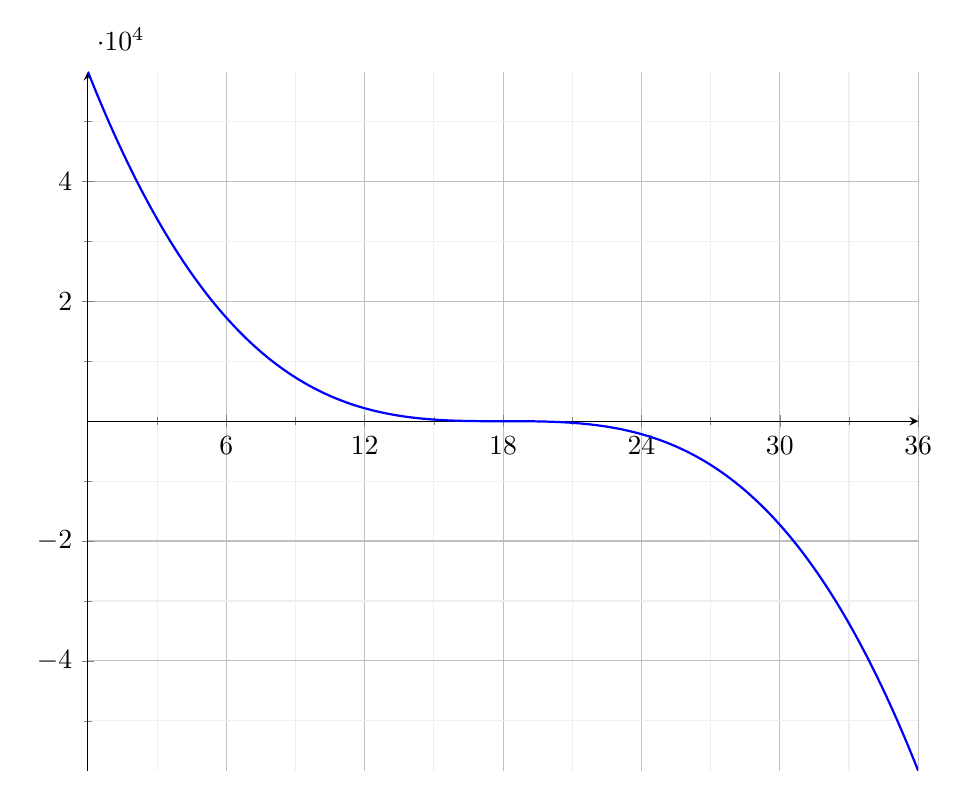
\begin{tikzpicture}
					\begin{axis}[
						axis lines=center,
						xtick distance=6,
						grid = both,
						minor tick num=1,
						major grid style={lightgray},
						minor grid style={lightgray!25},
						width=1\textwidth]
						\addplot[domain = 0:36, samples = 200, smooth, thick, blue] {-10*(x-18)^3};
					\end{axis}
				\end{tikzpicture}
			}
			\caption{Cubic function}
			\label{fig:evaluation--suts-fitness-function-cubic}
		\end{subfigure} &
		
		\begin{subfigure}{.5\textwidth}
			\centering
			\resizebox{0.7\columnwidth}{!}{%
				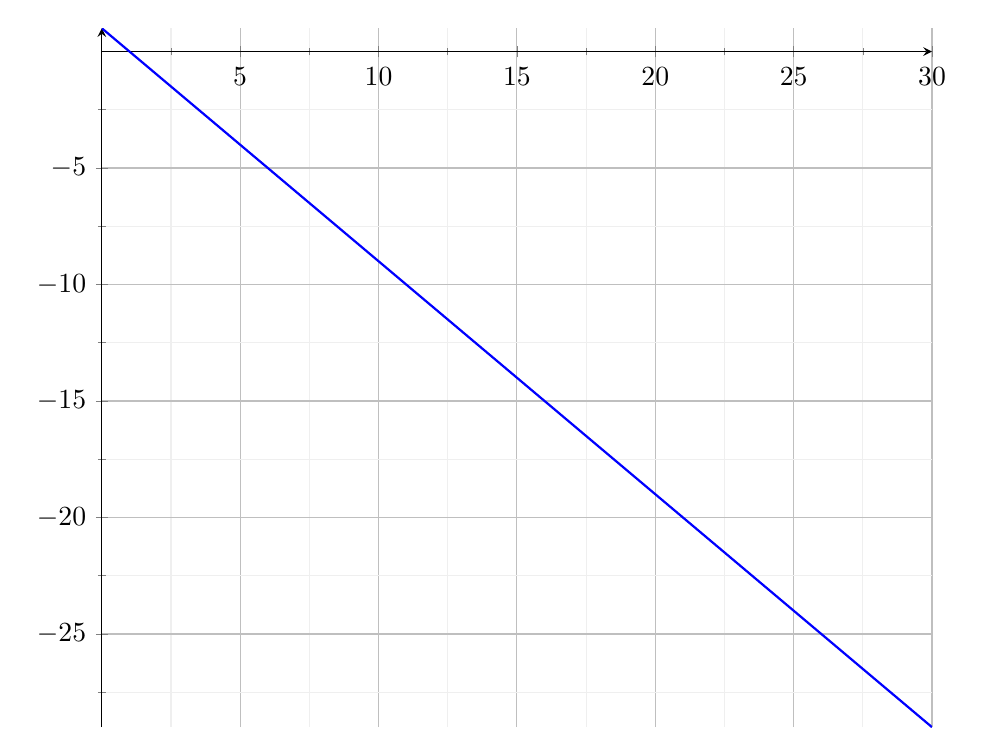
\begin{tikzpicture}
					\begin{axis}[
						axis lines=center,
						grid = both,
						minor tick num=1,
						major grid style={lightgray},
						minor grid style={lightgray!25},
						width=1\textwidth]
						\addplot[domain = 0:30, samples = 200, smooth, thick, blue] {-x+1};
					\end{axis}
				\end{tikzpicture}
			}
			\caption{Normalized function (before normalization)}
			\label{fig:evaluation--suts-fitness-function-before-normalized}
		\end{subfigure} & \\
		
		\begin{subfigure}{.4\textwidth}
			\centering
			\resizebox{0.9\columnwidth}{!}{%
				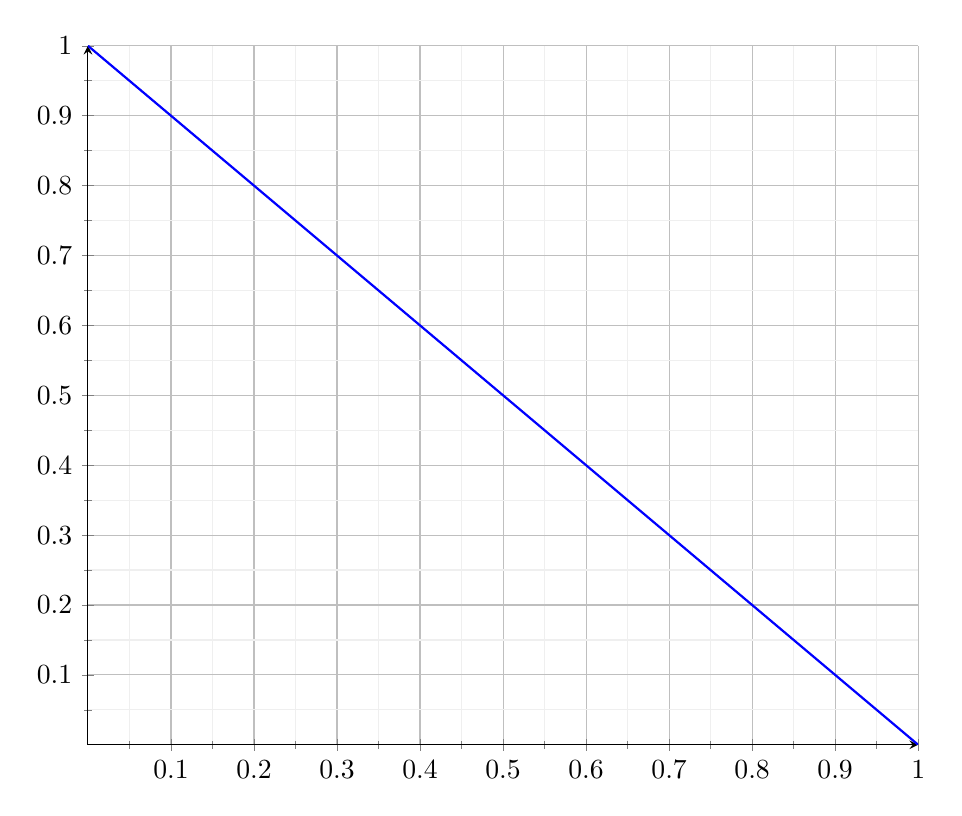
\begin{tikzpicture}
					\begin{axis}[
						axis lines=center,
						grid = both,
						minor tick num=1,
						major grid style={lightgray},
						minor grid style={lightgray!25},
						width=1\textwidth]
						\addplot[domain = 0:1, samples = 200, smooth, thick, blue] {-x+1};
					\end{axis}
				\end{tikzpicture}
			}
			\caption{Normalized function}
			\label{fig:evaluation--suts-fitness-function-normalized}
		\end{subfigure} &
		
		\begin{subfigure}{.5\textwidth}
			\centering
			\resizebox{0.7\columnwidth}{!}{%
				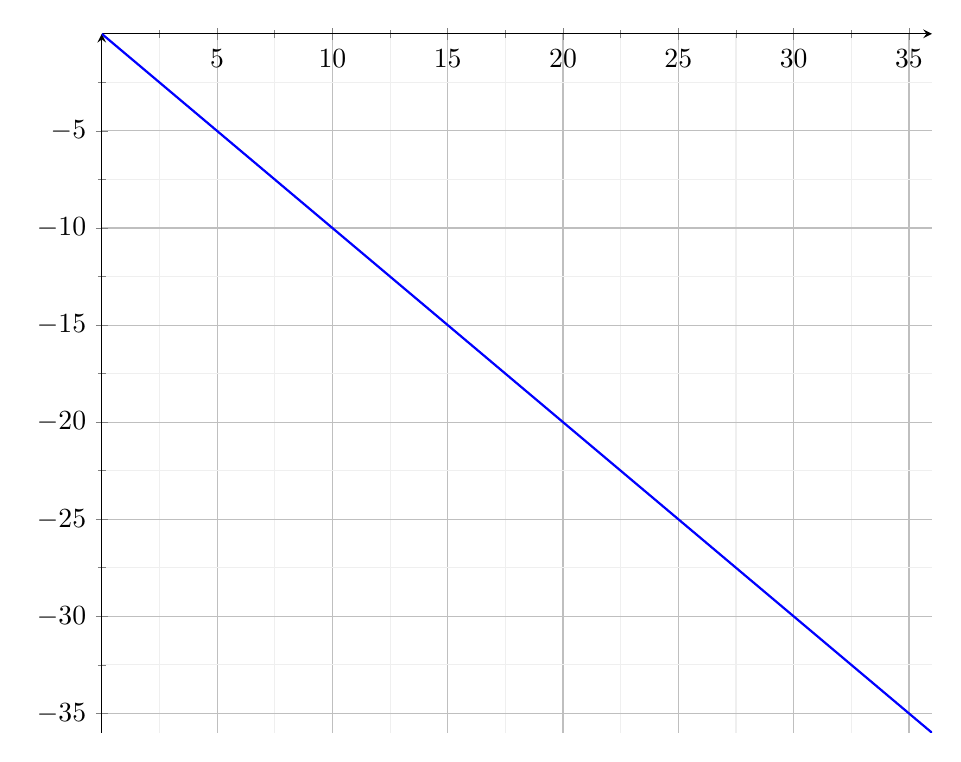
\begin{tikzpicture}
					\begin{axis}[
						axis lines=center,
						grid = both,
						minor tick num=1,
						major grid style={lightgray},
						minor grid style={lightgray!25},
						width=1\textwidth]
						\addplot[domain = 0:36, samples = 200, smooth, thick, blue] {-x};
					\end{axis}
				\end{tikzpicture}
			}
			\caption{Linear function}
			\label{fig:evaluation--suts-fitness-function-linear}
		\end{subfigure}
	\end{tabular}
	\label{fig:evaluation--suts-fitness-function}
	\caption{Components of the fitness function}
\end{figure}

\paragraph{Function approximation}
\label{par:evaluation--suts-function-approximation}

We implemented two model inferrers to approximate the \gls{EWTaBS} function (\cf Figure~\ref{fig:reference-architecture--architecture}). In both cases, the data points used as samples come from the genetic algorithm described in Section~\ref{par:evaluation--suts-evolutionary-optimization}---\emph{Evolutionary Optimization}. Since the genetic algorithm explores the solution space, from an evolutionary viewpoint, the metrics computed as part of the fitness function will provide a more accurate approximation over time. The first inferrer is based on function interpolation and uses natural bicubic splines. The second inferrer uses symbolic regression as follows. The inputs to the algorithm are the collected data points, which are of the form (\emph{number of buses}, \emph{headway design}, \emph{average \gls{EWTaBS}}), and a set of terminals that represent possible operators to apply during the space exploration. Based on trial and error experimentation, we arrived at the following list of operations: addition, subtraction, multiplication, exponentiation and square root. We configured the genetic algorithm to use the mean square error as loss function with a maximal tree depth (\ie{height}) of 5. Additionally, we specified three possible stop conditions: a minimum acceptable estimated error of 0.01, a total number of 10,000 generations, and a maximum execution time of 1 minute. To alter the offspring population we used a single node crossover with a 10\% probability and a mutator with a 1\% mutation probability.

In our experience, the symbolic regression algorithm will not always converge to a successful result. In most cases this happened because the stop condition (\eg{the number of iterations}) was triggered before the algorithm converged, thus, failing to reach an acceptable estimated error. Since this is a risk inherent to evolutionary optimization, we use the interpolated function as a fallback mechanism. This is because function interpolation guarantees termination and its estimated error highly depends on the density of the samples. Therefore, it is likely to improve over time.



\subsubsection{Multi-Adjustment Mechanism (\acrshort{am})}
\label{subsubsect:evaluation--suts-adjustment-mechanism}

Our implementation of the \gls{am} finds the argument to the reference function (\ie{the inferred function described in Section~\ref{par:evaluation--suts-function-approximation}---\emph{Function Approximation}}) that best approximates a given target value (\ie{the control objective}). For example, given a desired \gls{EWTaBS} of 5 minutes, the \gls{am} minimizes the distance between the reference function and the point $(0, 5)$, where the first argument is the headway design. That is, the function $d(x)=\sqrt{(x-0)^2+(f(x)-5)^2}$, where $f(x)$ is the reference function.

We used the gradient descent method to minimize the aforementioned distance equation. To do so, we implemented automatic differentiation of both the reference and distance functions. We only implemented one parameter estimator. However, other implementations would only differ in the optimization part.

%TODO T5 We only implemented the AM, not the run-time validation part - no way to evaluate with real system (future work)

\subsubsection{Application Scenario: Model Identification and Run-Time Adjustment}
\label{subsubsect:evaluation--suts-application-scenario}

The results of the performed evaluation comprise two parts. The first one concerns the effectiveness of the \gls{mim} to approximate the \gls{EWTaBS} function. The second one is about the \gls{am}'s ability to select appropriate parameters for the same function such that the transportation system meets its goal (\ie{to achieve a target \gls{EWTaBS}}).

The genetic algorithm was configured to explore the evolution space. As a result, it varies the number of buses and the headway design without describing a particular direction. Figure~\ref{fig:evaluation--suts-overall-performance} shows the overall fitness performance over (simulated) time. Both figures~\ref{fig:evaluation--suts-performance-exploration} and~\ref{fig:evaluation--suts-performance-optimization} plot the fitness value of the best chromosome for each generation. For comparison, we have included Figure~\ref{fig:evaluation--suts-performance-optimization}, which displays the performance of the genetic algorithm when configured to optimize the fitness value. The chart only displays 50 generations because the algorithm quickly converged. These two modes of operation exemplify the purpose of the \gls{mim} and the \gls{am}. The first one concentrates on generating enough information to synthesize active knowledge. The second one is concerned with finding appropriate control parameters regardless of the contextual situation. In fact, the density of the generated data points dictates how reliable are the inferred models.

\begin{figure}[h]
	\centering
	\begin{subfigure}[b]{0.49\textwidth}
		\includegraphics[width=\linewidth]{fig/evaluation/reference-architecture/charts/overall_fitness_performance.pdf}
		\caption{Exploration mode}
		\label{fig:evaluation--suts-performance-exploration}
	\end{subfigure}
	\begin{subfigure}[b]{0.49\textwidth}
		\includegraphics[width=\linewidth]{fig/evaluation/reference-architecture/charts/overall_fitness_performance_opt.pdf}
		\caption{Optimization mode}
		\label{fig:evaluation--suts-performance-optimization}
	\end{subfigure}
	\caption{Overall fitness performance over time}
	\label{fig:evaluation--suts-overall-performance}
\end{figure}

\begin{figure}[h]
	\centering
	\begin{subfigure}[b]{0.49\textwidth}
		\centering
		\includegraphics[width=\linewidth]{fig/evaluation/reference-architecture/charts/hcv_headway.pdf}
		\caption{Headway design vs \gls{HCoV}}
		\label{fig:evaluation--suts-results-hcv-headway}
	\end{subfigure}
	\begin{subfigure}[b]{0.49\textwidth}
		\centering
		\includegraphics[width=\linewidth]{fig/evaluation/reference-architecture/charts/hcv_ewt.pdf}
		\caption{HCoV vs \gls{EWTaBS}}
		\label{fig:evaluation--suts-results-hcv-ewt}
	\end{subfigure}
	\begin{subfigure}[b]{0.49\textwidth}
		\centering
		\includegraphics[width=\linewidth]{fig/evaluation/reference-architecture/charts/headway_ewt.pdf}
		\caption{Headway design vs \gls{EWTaBS}}
		\label{fig:evaluation--suts-results-headway-ewt}
	\end{subfigure}
	\begin{subfigure}[b]{0.49\textwidth}
		\centering
		\includegraphics[width=\linewidth]{fig/evaluation/reference-architecture/charts/fleet_ewt.pdf}
		\caption{Operating fleet size vs \gls{EWTaBS}}
		\label{fig:evaluation--suts-results-fleet-ewt}
	\end{subfigure}
	\caption{Correlation and behavior of independent variables and measured metrics with respect to the excess waiting time}
	\label{fig:evaluation--suts-results-correlation-variables}
\end{figure}

The simulation model was crucial to evaluate concrete combinations of parameters and estimate the metrics of interest. Figure~\ref{fig:evaluation--suts-results-correlation-variables} displays various abstract views depicting the behavior of independent and dependent variables. Figure~\ref{fig:evaluation--suts-results-correlation-variables} shows several charts depicting the correlation of independent variables and measured metrics with respect to the \gls{EWTaBS}. Figure~\ref{fig:evaluation--suts-results-hcv-headway} plots the effect of the headway design on the \gls{HCoV}. As expected, the direction of the regression line, along with the Pearson correlation coefficient, confirms that increasing the headway decreases the variation. In this case, the correlation coefficient and mean square error are valuable metrics to predict how reliable the approximated function can be. This can be useful when several model inferrers or parameter estimators are available. Figure~\ref{fig:evaluation--suts-results-hcv-ewt} depicts the effect of the \gls{HCoV} on the \gls{EWTaBS}. This result is consistent with the previous one: a large \gls{HCoV}, meaning that the headway is actually small, means that passengers will wait less time on average. This kind of linear relationship between the headway design and the \gls{EWTaBS} is also evidenced in Figure~\ref{fig:evaluation--suts-results-headway-ewt}. The clusters of points in Figure~\ref{fig:evaluation--suts-results-hcv-ewt} are a reason to suspect that the genetic algorithm may need to increase the crossover and mutation probabilities. Hyper-parameter optimization can help spread the generated headway values, thus potentially improving the accuracy of the approximated function. Finally, Figure~\ref{fig:evaluation--suts-results-fleet-ewt} shows that neither increasing nor decreasing the number of buses affects the \gls{EWTaBS}. This means that these two variables are not correlated (\cf{the Pearson correlation coefficient}), therefore the former should not be included in the distance function optimized by the \gls{am}.

Once the genetic algorithm has explored the adaptation space, the model inferrers can approximate the function. Figures~\ref{fig:evaluation--suts-results-headway-ewt-interpolation} and~\ref{fig:evaluation--suts-results-headway-ewt-regression} plot the approximated functions. On the one hand, the function approximated by interpolation produces accurate-enough results in areas with enough data density. However, there is a segment of the domain where the function returns a negative excess waiting time. The \gls{am} can include validations over basic assumptions such as this one. In this case, since a negative waiting time is impossible, a simple failover strategy may provide a better alternative. On the other hand, the function approximated by symbolic regression describes a more consistent, smooth curve. Such a curve is described by the function $f(x)=sqrt(9 + (((7 + 2x) + (x + sqrt(6 + ((8 + 2x) + ((4 + 2x) + (x + ((4 + 2x) + 9))))))) + (6 + ((9 + (x + ((6 + 2x) + 6))) + 2x))))$, with a mean square error of 62.37 seconds.

The \gls{am} is able to select a headway design correctly for a given a target excess waiting time. For example, an excess waiting time of 1.33 minutes is possible with a headway of 13.17 minutes. Of course, since the \glspl{cps} is in constant evolution, available \glspl{mim} will be constantly updating the reference models. The \gls{am} will always use an up to date reference input, decreasing the likelihood of unintended effects.

\begin{figure}[h]
	\centering
	\begin{subfigure}[b]{0.49\textwidth}
		\centering
		\includegraphics[width=\linewidth]{fig/evaluation/reference-architecture/charts/headway_ewt_int.pdf}
		\caption{Interpolated function using natural cubic splines}
		\label{fig:evaluation--suts-results-headway-ewt-interpolation}
	\end{subfigure}
	\begin{subfigure}[b]{0.49\textwidth}
		\centering
		\includegraphics[width=\linewidth]{fig/evaluation/reference-architecture/charts/headway_ewt_appr.pdf}
		\caption{Approximated function using symbolic regression}
		\label{fig:evaluation--suts-results-headway-ewt-regression}
	\end{subfigure}
	\caption{Approximated functions}
	\label{fig:evaluation--suts-results-approximated-functions}
\end{figure}

We have demonstrated the feasibility of our reference architecture by describing the model and implementation suitability of two prototypes for its major components. These components contribute to the achievement of dependable autonomy and operational resiliency in the design of \glspl{scps}. Our experimental results show that the \gls{mim} was able to approximate a function to describe the \gls{EWTaBS} using two estimators, based on cubic interpolation and symbolic regression (\cf Figure~\ref{fig:evaluation--suts-results-approximated-functions} and Section~\ref{par:evaluation--suts-function-approximation}). For this, the \gls{mim} exploits its exploration and optimization capabilities to synthesize and examine the effectiveness (\cf Figure~\ref{fig:evaluation--suts-results-correlation-variables}) of alternative configurations of the system (\ie through the genetic algorithm described in Section~\ref{par:evaluation--suts-evolutionary-optimization}---\emph{Evolutionary Optimization}). In other words, the \gls{mim}  is capable of synthesizing active and passive knowledge in the form of data, executable models or functions. These artifacts are useful for considering adaptation scenarios and evaluating their possible outcomes. Consequently, this component constitutes a baseline from which the adaptation and operational spaces are eventually devised and evaluated before their manifestation. We showed how this transition from evolution to adaptation manifests in our reference architecture using our second prototype, the \gls{am}. This contributes to the realization of our envisioned continuous engineering cycle.

The results obtained in this study constitute a promising step forward toward the achievement of \glspl{suts} and related types of autonomic \glspl{cps}. Our reference architecture promotes the exploration and validation, and exploitation of system adaptations at run-time (\cf Section~\ref{subsubsect:evaluation--suts-model-identification-mechanism}). This contributes to increase the dependability of control actions by providing guarantees about their potential effectiveness in managed systems. Moreover, our architecture delineates the way models can evolve at run-time to face the challenges associated with managing dynamic real-world entities (\cf Sections~\ref{par:evaluation--suts-function-approximation} and \ref{subsubsect:evaluation--suts-adjustment-mechanism}). With this, we expect to enhance overall system resiliency by enabling the system to mitigate run-time conditions that can not always be anticipated during design time.


\section{Chapter Summary}

This chapter presented the evaluation of our contributions. We conducted functional, experimental and qualitative proof of concept validation of representative elements from each contribution. The two case studies we presented previously in Chapter~\ref{chapter:contribution-overview} guide the validation concerns we addressed.

Based on the infrastructure management case study, we validated functional concerns of our continuous software evolution pipeline. We conducted this validation considering two application scenarios, namely: assistance with knowledge acquisition from deployed resources, and prevention of configuration drift for \gls{iac} specifications. In both cases, we described implementation details of our functional prototypes and walked through the steps to demonstrate how our implementation contributes to achieve the validation scenario. In the first case, we showed the process to generate the \gls{iac} template and instance corresponding to the deployed resources. In the second case, we described the functionalities of our prototype addressing configuration drift. Based on these application scenarios, we validated the soundness and feasibility of our evolution pipeline.

% TODO Add more details here
We also evaluated our self-improvement feedback loop based on the infrastructure management case study. We conducted an experimental validation of our proof of concept focused on the exploration of software architecture variants. We described implementation details, experimentation setup, and experimentation results. Our results evidenced the capacity of our self-improvement feedback loop to contribute to the managed system's long-term evolution. Based on the validated application scenario, we demonstrated the feasibility of our approach.

%We also evaluated our self-improvement feedback loop based on the infrastructure management case study. We conducted an experimental validation under two application scenarios, namely: exploration of software architecture variants, and exploration of infrastructure variants. In both cases, we described implementation details, experimentation setup, and experimentation results. Our results evidenced the capacity of our self-improvement feedback loop to contribute to the managed system's long-term evolution. Based on these application scenarios, we validated the feasibility of our approach.

In addition to functional and experimental validation, we validated qualitative concerns of our continuous evolution process, as well as its contribution to reduce the two discontinuities we described in Chapter~\ref{chapter:contribution-overview}. Based on the \gls{suts} case study, we evaluated our run-time evolution reference architecture as follows. We conducted a functional validation of our reference architecture focused on an application scenario regarding model identification and run-time adjustment. We described implementation details of our prototype, including: the modeling layer, which includes a graph-based topology of the transportation system, and statistical distributions for bus and passenger arrival; a proof of concept implementation of the \gls{mim} based on symbolic regression and function interpolation; and a proof of concept implementation of the \gls{am} based on gradient descend. Based on this scenario, we showed the consistency and feasibility of our reference architecture for guiding software architects on how to apply it for engineering \glspl{scps}. We validated the prototypes using concrete dependability and resiliency domain-specific concerns, such as the cost associated with a particular operating fleet size, the average \gls{EWTaBS} per passenger, and the \gls{HCoV}.

The next chapter summarizes the work we presented in this dissertation. It highlights our contributions and discusses potential future work.
